\protect\hypertarget{titlepage.xhtml}{}{}

\protect\hypertarget{index_split_000.html}{}{}

NO. 6 \textbar{} Atsuko Asano

\protect\hypertarget{index_split_001_split_002.html}{}{}

\hypertarget{index_split_001_split_002.htmlux5cux23calibre_pb_0}{%
\subsection{Volume
6}\label{index_split_001_split_002.htmlux5cux23calibre_pb_0}}

\emph{Where did you come from? Where were you born?}

\hypertarget{index_split_001_split_002.htmlux5cux23calibre_pb_1}{}

\hypertarget{index_split_001_split_002.htmlux5cux23calibre_pb_0}{}

\hypertarget{index_split_001_split_002.htmlux5cux23calibre_toc_2}{%
\subsection{CHAPTER
1}\label{index_split_001_split_002.htmlux5cux23calibre_toc_2}}

\subsubsection{'Twere best not know myself}

\emph{To know my deed, 'twere best not know myself.}

\emph{Wake Duncan with thy knocking! I would thou couldst!}

\emph{-Macbeth Act II Scene II~}

He heard the sound of the wind. It was a dry, sorrowful sound.

It can't be...

Shion stopped his feet, and blinked slowly. It was dark. Even when his
eyes were accustomed to darkness, the gloom only reflected into his eyes
as gloom, and was entirely painted black. And of course, there was no
wind blowing.

Here, they were at the bottom of the earth.

A place in the bosom of No. 6―precisely, a place of darkness. The
basement of the Correctional Facility. Of course there would be no wind
blowing. There was no way he could have even heard its sound. Yet he had
definitely heard a high-pitched whistling. It was for a mere instant,
but he had heard it.

It wasn't a sound he had heard before in No. 6, where he had been living
only a short while ago. It wasn't a breeze that gently shook the
abundant canopies, nor was it something that wafted the sweet fragrance
of flowers to him. It was―

The wind of the ruins.

It was the cry of the wind that whistled through the remains of the
dilapidated hotel in a corner of the West Block. It was a cold wind.
Every time he felt it against his body, he remembered feeling like he'd
been chilled to the marrow of his bones. And indeed, people like the
elderly who collapsed on the road, unable to move, or children who had
been depleted of energy from starvation, were whipped by this frigid
wind and eventually froze to death. It was a cruel and ruthless winter
wind.

But he missed it.

He yearned many times more for the chilling wind that swept through the
ruins over the gentle, harmless breezes in No. 6.

What was Inukashi doing now? Was he simmering leftovers in the big pot,
briskly making food for his dogs? Was he busy tallying up his earnings
for the day? Inukashi, with his tan skin, ink-black hair and wiry body.

He had left a baby in Inukashi's care. He had thrust a small infant boy
upon him against his will.

Cut the crap, Shion. I'm operating a business here, my hotel. I'm not
running a non-profit orphanage.

Shion could imagine his face, scowling in disgust.

Sorry, Inukashi. I didn't have anyone else to depend on. I had no other
choice but to cling and beg for your help.

Tsk.

Inukashi clicked his tongue.

Pain in the ass wherever you go, aren't ya? Fine, I'll take it. Even I
have the heart to feel a bit of compassion. But it's a tiny one, and
even a dog would turn its nose up at it. No choice, though. This baby's
someone my own dog has risked its life to protect. I can't just throw
him away.... Look at me, I'm a pushover. Makes me sick of myself, even.

Inukashi, my gratitude.

Doesn't make me happy one bit to have any of your gratitude. Doesn't
give me any gain. Shion, I'll take the baby for now. Got it? Only for
now. You better come pick him up. You decided to take this guy in. You
gotta raise him. Understand? You better come pick...

"Shion."

Nezumi turned around, and called his name. He could clearly see the pair
of lustrous grey eyes. Even in this darkness, Nezumi's eyes both sucked
light in, and released it. Or― Shion let his thoughts wander.

Or could I still render those eyes, even if there was no light, even if
I was in complete darkness without a single ray to illuminate my way?

"Don't stop walking. Keep right behind me."

"Oh―right. Sorry, I was spaced out a bit."

"Spaced out?"

"I thought I heard the wind blowing. Like the wind that used to blow
against Inukashi's ruins... I know I'm just hearing things, but―Nezumi."

"Hm?"

"I wonder what Inukashi's doing right now."

Nezumi blinked. Shion could make him out catching a breath.

"You've got guts."

"Huh?"

"Not just anyone can space out in a situation like this. There are
probably tons of people who go into shock from nerves, but to be able to
hear the wind blowing, or casually think about other people―that's
colossal. The amount of guts you have probably puts you in ranks with
the gods. You will let me worship you every day, won't you, once in the
morning and in the evening?"

"Are you being sarcastic?" Shion said flatly.

"Why, never," Nezumi said. "I haven't got the courage to smart-mouth a
god. I'm genuinely impressed. But―"

Shion was grabbed by the arm. It hurt. He felt Nezumi's fingers digging
into him. He knew how much strength those fingers held, despite how
slender and almost delicate-looking they were. So many times Nezumi had
clenched his arm, making him wince in pain. So many times he had grabbed
his arm and pulled him up. Again and again, countless times―from death
to life, from despair to hope, from fiction to reality, Shion had been
able to crawl up and out thanks to these fingers.

"From now on, be a bit more of an earthly coward. Don't give a damn
about Inukashi. Only think about protecting yourself."

"Got it."

"―Do you really get it?"

"I do―probably."

"Probably, huh. Nothing reassures me less." Nezumi gave a sudden laugh.
It was small, but it was lighthearted and filled with mirth. "Look at
the conversation we're having, in this place, in this situation. The
epitome of flippancy, I think, both you and me. Maybe I'd be able to
join the gods if I hang around you more."

Then his tone suddenly changed, into one that was heavy and severe. His
fingertips dug in with even more force.

"No matter what happens, don't stray from me. Keep up with your own
strength. I told you before. I won't say it again."

Shion nodded. Nezumi turned his back and resumed walking, either having
seen or felt the slight inclination of Shion's head in reply. The figure
before him wouldn't turn back around as easily. Shion knew that well,
too.

If he wasn't desperate enough to live, if he didn't greedily latch onto
life, then Nezumi would not turn to him.{[}2{]}

Nezumi would never revere a flippant and unobservant god. Shion inhaled
a breath of darkness, and placed his foot forward.

A small path continued up a slight slope in the crack between the
boulders. It was just wide enough for an adult to get through. It might
even be narrower than the former passageway, cased in concrete with
small light bulbs at equal intervals. It wasn't a long journey, but
twists and turns made it that much harder to walk through.

But at least―

Shion wiped his sweat with the back of his hand.

But at least it doesn't smell like blood here.

The air was absent of the bloody stench that had filled the other
passageway. There were no screams or groans of the dozens of people
dying―being murdered.

There was only darkness.

Even if this were only to last for a short moment; even if there was a
reality beyond Shion's imagination waiting for him beyond the darkness,
as it had always done, he would not have to breathe the stench of people
being unfairly and pitilessly obliterated.

He was grateful. As if he had encountered an oasis in a desert―he was
grateful.

You're naive.

He chewed his bottom lip.

Nezumi didn't even have to tell him. He was so very much naive.

I just can't smell it. I just can't hear it. I just can't see because of
the wall that divides us.

But it's still happening right beside me.

The reality that dozens of people―including newborns―were being unfairly
and pitilessly obliterated, still existed on the same stretch of land
that Shion stood on, right here, right now.

Just because he couldn't smell it, just because he couldn't hear, just
because he didn't see, didn't mean that it didn't exist. Just because he
had arrived at an oasis, it didn't mean the desert had disappeared.

I'm naive; I'm idealistic. He couldn't help but make excuses. He
couldn't help but try to forget the wrath he had felt when he had
witnessed the brutality. He wanted to avert his eyes from grisly things.
He was trying to curl up and lend himself fully to the comfort of
falling into an ignorant slumber.

I am naive. And I am weak.

He traced the rocky wall with his hand, and did his best to keep up with
Nezumi.

What was important right now was to follow him. And I've always followed
him. He had walked down a nighttime path for the first time in the West
Block. He had torn through it, even. If it weren't for that experience,
he would probably not be able to walk through the oppressive darkness
now that seemed to crush his very eyeballs.

In that sense, I've toughened up a bit, he told himself. Believe. You've
got your own kind of strength stored up inside you. Believe yourself
wholeheartedly. It was easy to fall back to self-loathing, and wallow in
defeat―but it was meaningless. Believing yourself was strength. With
this strength as fuel, as a weapon, one could overcome innumerable
difficulties.

Shion funnelled his concentration into the soles of his feet, and moved
forward one step at a time. He met a light. It was dim. It was gradually
beginning to lighten before his eyes.

Nezumi's figure glided into that dim light as he watched from behind.
Shion quickened his pace.

"Oh―" his breath caught in his throat.

They had emerged into a spacious chamber. It was much more spacious than
where Nezumi and the sand-coloured man had fought. The ceiling was
lofty. It looked almost three storeys high. The same rugged boulders
jutted out from all around.

This place is a naturally-occurring series of caves, huge and complex.
Nezumi had told him. Then this must be a chamber that nature had
created. Candles were lit here and there in the crevices, and they were
not the only thing: lamplight also winked in some places. They were all
dim, but warm, sources of light. They were beautiful, too―like small
flame-coloured flowers blooming in the alcoves of rock.

Alcoves?

Shion squinted. He baited his breath, and squinted as hard as he could.
He baited his breath more.

A shadow moved.

One, two, three, four.... They were not mice; those were not small
animals. Numerous shadows were moving around. They stood on two legs,
and were whispering to each other. On two legs, whispering....

Humans!

The lump he had swallowed stuck in his throat. His heart raced.

Humans. There are humans here. They're peering out at us from the
alcoves. Humans. If he squinted even more, he could see a large cavern
yawning its large mouth from behind the lit candles in the crevices. So
there were tunnels even further on inside these caves. The people had
probably crawled out from there.

Shion couldn't make out each individual figure with his eyesight, but he
could tell that they varied in height and build.

Were there men and women, both adults and children? All of them
identically leaned forward, and were gazing down upon them. Shion felt
like he could see each person's eyes glinting dully if he stared long
enough.

"Nezumi, these people..."

"Who do you think they are?"

"Oh―survivors. They must be people like us, who've managed to escape the
execution grounds."

"Wrong." Nezumi shook his head. It was a languid gesture, unusual for
him. "They've lived here way before that."

"Way before... what do you mean?"

"You'll see in a bit."

'You'll see in a bit'―I guess you're right.

You will see. As long as you have the will and the strength.

Shion clenched his fist. It was easy to question. He had always been
asking questions up until now. He had always instantly, so easily,
begged Nezumi for the right answer without trying to decode the reality
that appeared before his eyes.

It won't work anymore.

He would find the answer himself. He would grasp it. He would decode it.
Other people were other people, even someone as close as Nezumi. He
would not be able to render the truth if he kept leaning on other
people's words. He would not be able to face off with a reality that
surpassed his imagination. He would not be able to stay equals with
Nezumi.

He had to render it himself.

Nezumi dropped his gaze from Shion. His grey eyes clouded over. Clearing
it away with a blink, Nezumi swept his hand aside in a smooth gesture.
It was a graceful move unique to him.

"Look, isn't it spectacular? Everyone has turned out for the welcoming
parade."

"Famous even in a place like this, aren't you?"

"―Idiot. Shion, this is your welcoming."

"Mine?"

"You're the spectacle here. It's unheard-of for an outsider to come
bursting in. And a No. 6 resident at that."

"Former resident," Shion corrected. "I'm not one anymore. I threw my ID
card away a long time ago. I'm not a citizen of that city."

"Don't get hung up about it. It was just a form of expression."

"I will be hung up," Shion said stubbornly. "It isn't 'just' an
expression. I'm not as weak as you think. I'm not attached to No. 6."

Maybe it was bravado. But Shion squared his shoulders the best he could.

I am weak. My mind and body are all too fragile. But nothing can shake
my resolve. Nothing can confuse my feelings. My resolve to live not
within, but outside the city; my feelings of wanting to live together
with you; nothing can shake them, nothing can muddle them.

"Who said you were weak?"

"You always say so."

"Never. You're a superpower. You just overwhelmed me with your
brilliance back there. It's quite something... I'm even more impressed
now. I certainly am." Nezumi shrugged. "And I would never have thought
you would trip me up at every petty word and start complaining about it.
In this situation much less."

Skrit, skrit, skrit.

A sewer rat crawled up Shion's body, and sat on his shoulder. It was
quite heavy compared to Hamlet or Cravat. And it smelled rotten. But it
twitched its nose and tilted its head to the side in the same way.
Another one crawled onto his other shoulder. It stuck its head into
Shion's snowy hair, and nuzzled its face into it. Yet another one―this
time, a baby rat―rubbed itself against his feet. One more came, and
still another.

The rats scurried up and down Shion's body, chirruping affectionately.

Skrit, skrit, skrit, cheep cheep cheep.

Chit chit chit. Chit chit chit.

"Hey, cut that out," said Shion, suppressing a laugh. "I'm not a
playground slide. Stop that, it tickles!" Shion gave his body a shake.

The air buzzed. The darkness rippled uneasily. Shion could feel the
presence of the rock dwellers: breaths sucked in, inaudible whispering,
shifting bodies, furtive glances.

"An intriguing child."

A voice came raining down from above. It was a low voice, but it rang
out clearly. It wasn't quite the level of Nezumi's singing, but it was
deep, soothing, and flowed into his ears comfortably. Was it the same
voice as a few moments ago? The voice that had come floating down from
the black painted void?

'Let us hear your story.' Was it the same voice as that?

He looked up.

He saw a figure of a man seated in a chair in the middle of an alcove,
in a spot that was jutting out like a balcony. At least... he thought it
was a man. It looked like... an elderly man with long white hair and a
long white beard, clad in a long gown-like garment. It was too dark to
get a good look at his face.

"An intriguing child. You haven't stirred any animosity or apprehension
in the mice. Shall I ask you your name? What are you called?"

"I'm Shion."

"Shion―ah, a beautiful name."

"Th―Thank you. For, um, complimenting me," Shion stammered. "And you
are?"

"Me? What about me, Shion?"

"What is your name?"

Buzz.

The darkness rippled even more fiercely. The rats chattered on his
shoulders. Laughter rose. From alcoves in every direction, various kinds
of laughter rose, and showered down upon Shion.

Giggle, giggle, giggle.

Name, he says.

Giggle, giggle, giggle.

He asked for his name.

Giggle, giggle, giggle. Giggle, giggle, giggle. Giggle, giggle, giggle.
Giggle, giggle, giggle.

He had no idea why he was being laughed at. He had only asked for the
man's name. Why was that a cause for such derision?

Giggle, giggle, giggle. Giggle, giggle, giggle.

The laughter didn't cease. Shion turned to look at Nezumi, who was
standing at his side.

Nezumi stood unmoving. He wasn't smiling. Naturally. No expression
adorned his face. He was like a statue.

"Rou." A deep voice pierced through the rippling darkness. The noise in
the caverns was silenced immediately. An almost painful stillness fell,
like one you encountered in a forest when all the winds had died. In
this stillness, only the elder's words unfolded leisurely.

"Rou. That is what I am called."

"Rou―that's your name?"

"Perhaps, perhaps not. It may only mean 'old person'."

"So this is not your real name?"

Some moments of silence.

"Young one. No one here places importance on names. No one. Has Nezumi
not taught you that?"

Come to think of it―

Shion exhaled.

Come to think of it, I still don't know Nezumi's real name.

"Rou." Nezumi moved. He had taken a step forward. "I want you to hear
our story."

"Let us hear it." The elder straightened his posture in his chair. "You
have returned. We were never supposed to meet again, yet you have
appeared again before my eyes. Let us hear the reason."

"I'm grateful."

"Grateful? Nezumi, I see you have been grown weak and cowardly from
being buffeted by the wind outside. But no matter how weak and cowardly
you have become, I hope you have not forgotten the rules."

"Of course not."

"Those who have left this place must never return. You have broken that
taboo. You must recompense."

"I know. I'll pay the penalty. So listen to me, please."

The elder snapped his fingers. Although Shion had not noticed this
before, two long poles were attached to the legs of the elder's chair.
It was perhaps better called a palanquin than a chair.

Two men held the poles and hoisted the elder along with the palanquin.

His legs?

There was nothing filling out the lower part of the elder's gown. The
hem hung lifelessly. The elder had lost his legs from the knees down.
Both of them.

The palanquin with the elder in it began to descend from the boulders
slowly, as if slithering down the wall. A shadowy figure, whose long
hair was bound in a ponytail―a woman, evident from the outline of her
body―was sweeping the path in front of the palanquin with what looked
like a broom. She was like a forerunner for a procession.

There was a path. A path just wide enough for people to brush shoulders
as they passed. The slope was steep, yet the men walked steadily down
it, without missing a step.

It was not something naturally-occurring. Walkways had been carved into
the boulders by human hands. If he looked closely, paths spanned all
along the rocky walls; perhaps it was structured so that people could
come and go freely.

Is this... a settlement?

Shion took in his surroundings anew. At the same time, he set his brain
to work. Caverns, which were no doubt residences; paths on the boulder
walls; this chamber; the dark space that continued beyond this
chamber―and he could almost smell something being boiled or stewed. And
faintly, very faintly, he could feel a wind. Which meant the air was
moving, and this place was connected to ground-level. Here was a
settlement of humans.

An underground settlement?

He restrained his thoughts, which threatened to stray every which way.
He organized them, and searched for a coherent thread.

Nezumi had said that these residents of the dark were not people who had
survived the Hunt. It was perhaps so. An underground world, where no
sunlight would reach, would be too harsh of a condition for people to
live in. Humans were organisms that were adapted to life above ground.
It seemed implausible that one could keep living in a place where there
was barely any change in amount of sunlight, air current, and natural
surroundings. But before his eyes were those very people themselves, and
the signs of human residency.

The scene before him was clearly not something that had been created
overnight. He could gather that much. Had these people lived underground
for a long, long time, having established their settlement, and
gradually adapted this way? It was the only guess he could come up with.

Shion unconsciously let out a long sigh.

Remember this place. The basement of the Correctional Facility. What is
a settlement doing here? Is it a coincidence?

Maybe...

Shion's thoughts emitted frustrated sparks inside his head. No matter
how much he thought about it, he wasn't able to grasp it. He couldn't
set foot outside of the boundaries of speculation. But that was also why
he thought harder. He speculated. He devised theories of "what-if"s.
Desperately.

What if people had been living in this place for much longer―this place
that had been a series of large caves from the very beginning?

Aboriginals...

What if there had been people living on this land long before the birth
of the nation-state of No. 6?

The West Block area had once been a small but beautiful town. Many kinds
of people, Rikiga included, had resided there. His mother had been
there. And his father―though he had no memory of him or his face―had
also been there. The town had mutated, and became the mother from which
No. 6 was born. Except it wasn't the town that had changed, it was the
people. Under human hands, the massive walls of special alloy and the
enormous city-state had been born. Outside of the walls, the remnants of
the town became a barren wasteland known as the West Block. But that was
only the west side.

Was the western town the only place No. 6 had destroyed? What about the
northern mountains, the forests, the grassy plains that stretched from
south to east, the lakes and marshes that dotted the land from eastern
to western edge? Considering No. 6's geographical area, it was logical
to think that it had enlarged in all four directions, proliferating and
expanding...

A chill ran down his spine.

In the northern mountains, the southern plains, the eastern marshes.
Somewhere, a race of peoples unknown to Shion had once lived. And not
only one race. In the mountains, forests, and plains, people had carried
on their lives. In these caverns, too....

Aboriginals. A people who had taken up residence in the caves from a
time dating far back.

They had been people of a different kind of world than the town Rikiga
and his mother had lived in; they had probably stayed in their own
territory, as the "town people" lived in theirs, and had not had any
contact with them. Perhaps neither group was even aware of the other's
existence.

This stretch of land had once been a sprawling forest. On this planet,
there were only six regions which fulfilled the conditions adequate for
human life.

People built towns in those regions, and those towns eventually grew
into city-states. Learning from history's moral lesson, they had
abolished civil wars between the states. They agreed that a ban on all
military power was the bottom line for the continued survival of
mankind, and so, they had acted in accordance with the Babylon Treaty,
which called on the abandonment of all armies and weapons. Also in
accordance, each city had discarded its unique name, and adopted a
simple number as its title―from No. 1 to No. 6.

The six cities, while still respecting the uniqueness and independence
of each, nevertheless maintained strong ties, and were acknowledged to
be part of one nation; both political leaders and the populace agreed
that this was the mindset each and every one should have.

These lands are the only things left to us. Further destruction is not
permissible. War is evil. It leads everything to extinction. It
threatens our very existence. We must abandon all weaponry for the
future of humankind.

Under this ideology, we shall found six cities linked in friendship and
understanding.

From No. 1, to No. 6.

The sixth region had been blessed with natural conditions more
favourable than any other. Everything was utilized to the
fullest―nature's bounties, human intelligence, and scientific
technology―to build this utopian city, one rarely found throughout
history.

This was the birth of the Holy City of No. 6.

That was an outline of the history Shion had learned as an elite
candidate in his perfectly-equipped classroom.

His chill had gotten worse. He felt like he was frozen right down to his
fingertips.

If he closed his eyes―but even with them open―he could see images of the
Hunt flashing in the back of his mind. It was reality. Those were scenes
he had seen with his own eyes.

Barracks had been blown apart; tents had been torn down. Frantic,
fleeing people had been ruthlessly murdered. Men and women, both elderly
and young, and even infants had been indiscriminately vaporized. The
most modern weapons had attacked people who could only retaliate by
throwing rocks. It was a massacre if anything.

'Abandon all weaponry' indeed.

He had been biting his lip without thinking. The bloody taste spread
inside his mouth. He swallowed it with his spit. He did not know about
the other cities. But―but...

At the very least, he knew that No. 6 was on its way to becoming an
armed state with overwhelming military power.

\emph{Since when?}

He swallowed his bloody saliva again.

\emph{When did that city start to change? When did it begin to stray
from the policies and ideals of the Babylon Treaty? Since when... since
the beginning?}

Shion felt a gaze on him. His eyes met with Nezumi's. He felt like he
was being wrapped in an elegant grey cloth. The core of his body
pulsated. All the thoughts that had been swirling around in his head
came to a full stop.

A moment of pleasure.~

It was strange. Just the kind of light in Nezumi's eyes was enough to
make him feel like he was being pushed away or being embraced.

But now was not the time to be giving himself up to selfish and
indulgent emotions. People were easily swayed once they ceased to think.
They were too easily led along by the flow of other people's words and
the mindset of the times.

Nezumi would never embrace and protect anyone who avoided thinking, who
let himself simply be pushed along with the flow.

And besides, Shion thought as he lifted his chin. I don't want to be
protected by him. I haven't abandoned my thoughts. I'll keep decoding
the world around me and its workings in my own way. I will confront the
world in its true form, and look reality in the eye. That's probably
something you would call a battle, Nezumi.

Shion dropped his gaze from Nezumi, and meditated. He set his thoughts
in motion again.

Since when?

From the beginning?

Yes, from the beginning. Perhaps No. 6 had been removed from ideologies
of peace and co-existence from the very moment of its birth.

On this land, there had once been a people that had lived here long
before. No. 6 had invaded them. They had tried to dominate them in the
same way a starving beast devoured its prey and gnawed on its bones. By
doing so, it had expanded its boundaries, and established its
foundations as a city-state. Peace? Co-existence? It had laughed
contemptuously in face of these words, and with brute force, made the
surrounding areas its own.

Just as it had destroyed the West Block. Just as it had massacred its
people. Using overwhelming military force.

But still... what about the other thing? LEDs―light-emitting diodes.
LEDs lit up when electric current was applied to the joint between two
special semiconductors. They were man-made lights that didn't exist in
the natural world. Scientifically manufactured lights. Were they not
things that No. 6 had created? Or―or, rather, had some scientific
civilization existed which was at par with, or even more advanced than
No. 6? But if that was so, the civilization would probably not have been
invaded so easily. He did know that science was neither all-solving nor
almighty, however....

He didn't know. It was like walking in a fog. No matter how much he
pondered and contemplated, no matter how far he stepped in, he never
reached the truth. The more he thought, the further he ventured, the
more lost he felt. He couldn't get out of the labyrinth. His thoughts
wandered aimlessly.

He was frustrated.

Cheep.

The rat jumped down from Shion's shoulder. The little mice also hid
themselves in the boulder cracks.

What's wrong?

As Shion's gaze started to follow the little mice, he was suddenly
attacked from behind. A shadow twisted his arm up behind him. His mouth
was gagged. In the blink of an eye, he was bound up with rope. He was
shoved from behind. He fell with his hands still tied behind his back.
He rammed his shoulder on the ground.

"What was that for?" he shouted.

"Shion, keep quiet." Nezumi, also kneeling in ropes, shook his head at
him. "Don't resist. Stay quiet."

"But why―ow! The rope really hurts!"

"Let your body relax. Breathe out and loosen up. It'll feel a bit
better."

He did as he was told. Nezumi was right―he felt a bit better. Pretty
amazing, though. Capturing and binding us in a matter of seconds―oh, but
still―

"Not as good as you."

"What?"

"You'd have a better handle on it. Whether it be a rope, or a knife."

"Why, thanks for the compliment. I'm undeserving of the privilege,
really, to be complimented by you."

"I'm always in awe at your―gh." The rope dug into his neck. His breath
caught in his throat.

"Do not speak." A flat voice hissed at his ear.

Was it that man? The man with sandy-grey hair, skin, and eyes?

"Any more idle chatter, and I will wring your neck."

The rope tightened. He really felt like his neck was being wrung. His
airway caved in from the pressure. He felt like he was suddenly swelling
from the neck up. He couldn't breathe. It was painful.

"Knock it off," Nezumi said quietly. "Revenge for what happened back
there? Taking your frustrations out on an unresisting human? I see
you've picked up some low habits while we haven't seen each other,
Sasori."

The rope loosened. For an instant, Shion didn't know what was happening.
He threw himself out on the ground, and dissolved into a fit of
coughing. He heard the sound of flesh hitting the ground as if it were
crawling across it. He raised himself.

Nezumi was crumpled beside him. The man's foot landed on his shoulder.
He was wearing sandals that were woven out of what looked like thin
strips of bark.

"You too, Nezumi." The man's voice grew leaden. "Enough of your insolent
complaints. Do you not understand your place? Then it is only a matter
of making you understand."

The man's foot moved to kick Nezumi's shoulder.

"You are the ones who have trespassed from outside. You have no right to
protest if you get killed."

"Stop!" Shion twisted and yelled. Nezumi lifted his face, and shook his
head as if to tell him to shut his mouth. But he could not.

"You coward! You're just as Nezumi says. Tying us up and making it so
that we can't fight back, and then beating us―it's low, it's filthy!"

"Shion." Nezumi grimaced. Several streams of blood ran from his temple
down his cheek. Shion clenched his stomach, and stared up at the man.

"What is this place? No. 6?"

"No. 6, you say?" The man's whole body quivered. His sand-coloured eyes
glinted sharply. The light seemed almost murderous. But Shion was not
about to be silenced. He was also trembling, but not with fear. It was
with wrath. Wrath boiled within him.

"It's true. You're just the same. What you're doing is no different from
No. 6. You oppress the weak by force. You inflict pitiless violence. How
are you guys any different?"

"I'm not really weak, just saying," Nezumi shrugged with his hands still
tied behind his back. "Shion, I get what you're trying to say. Just
leave it at that. Say any more, and you'll be kicked to death. Kicking
is this old man's specialty."

"I will kill you," the man growled. "You are a demon. A wicked bringer
of misfortune. If I do not dispose of you now, you will only bring
catastrophe upon us."

"A sharp eye, Sasori," Nezumi sighed exaggeratedly. "You're spot on. A
catastrophe, indeed. Of the highest class."

"Nezumi, what do you mean 'catastrophe'? ...You mean I am?"

"You are," Nezumi chuckled lightheartedly.

"He is evil," the man continued. "He wears a demonic aura like a cloak,
and carries misfortune wherever he goes. I can tell. Nezumi, you said he
was a resident of No. 6."

"Former resident, to correct you. He was inside the city up until just
recently."

"That must be why he is so evil. He is... like No. 6 itself."

Nezumi narrowed his eyes. The tip of his tongue licked the blood on his
lips.

"No. 6 itself, huh.... I see. That's how he appears to you."

"I know," the man answered. "I can tell. I must kill him. I must dispose
of him before it is too late. If not..." The man took a step forward.
Shion shrank back without thinking. The man was radiating such a
murderous intent that he could not help but recoil.

He's serious....

This man is serious about killing me.

The man took another step forward, but suddenly spun in a somersault and
crashed to the ground. Nezumi had tripped him.

Nezumi was up in a flash. The ropes slid to the ground. It was like a
magic trick. In his hand was a small knife.

The man tried to get up, but was stopped by Nezumi's knee digging into
his stomach. The man let out a muffled groan. He bent backwards from the
pain, leaving his throat defenseless; a blade was soon pushed up on it.

"We worked hard to get here. I won't have you disposing of him that
quickly."

"Why... did you bring... such catastrophe?" choked the man. "Do you plan
to destroy us all?"

"The opposite." Nezumi's lips curled. "I want to send No. 6 to its
grave. That's why I brought him."

"No. 6? Does that boy have the power to?"

"Who knows. We don't know until we try. I can't let you kill him before
we even test it out. That jealousy of yours, by the way: a little
embarrassing, don't you think?"

"Jealousy?"

"Yeah. You're jealous of Shion. He's got your rats in the palm of his
hand like it's nothing. You're jealous. Am I right?"

There was a heavy grinding sound. The man was gnashing his teeth.

"Nezumi... just as unpleasant as you used to be. It irritates me. I will
strangle you to death first."

"What a splendid promise. I can't wait. But before that―" The wan smile
disappeared from Nezumi's mouth. A drop of blood that had slid down his
chin dripped on the man's chest, and coloured it red. "Let's have you
swear, Sasori. Swear that you'll never lay a finger on Shion again."

The blade of the knife jerked. The man's throat contracted as well.

"Swear it."

The man fell stubbornly silent.

"That is enough." A gentle voice rang out. It even held a hint of a
laugh. "You have not changed, Nezumi. Neither your skill with the knife
nor your sarcastic way with words has deteriorated. I daresay it seems
to have become even more polished."

The elder on the palanquin was smiling with the same benign air as his
voice. The palanquin was lowered steadily.

"Rou."

"You have grown. I can barely recognize you. I would never have thought
I could encounter you as a grown man."

Nezumi released the man and knelt down. The knife spun once in his hand
before disappearing. This too, was like witnessing a magic trick. The
man muttered something, and gnashed his teeth some more. Rats raced over
Shion's lap.

"I believed that you had left long ago for a land far away. Did I not
command you to do so? To leave this place behind, forget everything,
throw everything away, and to live freely?"

"Rou, please listen to me."

"You should never have returned. Regardless of what happened, you should
never have come back."

"I can't be free." Nezumi clenched his fingers hard. "As long as No. 6
exists, I can't be free. I can't forget it, nor can I throw it away."

"Nezumi."

"You should know. No. 6 still exists. It's still here. How can I be the
only free one? It's impossible."

"I have told you not to become trapped. I have told you to live
unfettered. If you did not, you would not be able to survive; I
understood this well. That was why I released you into the outer world.
But to think that you would come back..."

"I've realized."

"Realized?"

"I've realized your words were nothing but white lies."

The air wavered in agitation. Voices which were barely voices traversed
between the people nestled in the rocky walls, looking down at them.

"Your words were white lies. False. There was no way I could live
without being trapped. On the contrary, I had to be trapped. Even if I
deceived myself, pretending I was free, I would still be in chains
anyway. From now on, I'll acquire real freedom with my own hands. I'll
set myself free. That's why I came back."

"Is this freedom you speak of fighting with No. 6?"

"It means fighting and winning. Erasing it clean from this land. The day
I see the Holy City arrive at its end is when I'd be free for the first
time. I'd be able to live a truly free life. I would be able to leave
this place... of my own will."

"Nezumi!" Shion yelled without thinking. As he yelled, grabbed Nezumi's
shoulder. "What do you mean by that? Leave this place? What―"

"Shion." Nezumi's eyes blinked rapidly. "The rope... how did you―?"

"Huh?"

"The ropes. How did you get out of them? You don't have a knife on you."

"What? Oh, the rats chewed them apart for me."

"The rats? No way, you must be―"

Shion thrust an end of the rope to Nezumi, and waved it before his eyes.

"Look. They all chewed at it together. It happened in no time.
Impressive, isn't it?"

Nezumi's eyes flitted to the jagged end of the chewed rope before
furrowing his brow.

"You have that much control over those rats?"

"Me? No, of course not. I couldn't pull tricks like that. The rats did
it on their own. They're all very kind and intelligent," Shion said
proudly.

"Kind and intelligent, huh. So your rats chew apart the ropes their
master has tied. He's right; they are kind and intelligent. You've
trained them to be very well-behaved, Sasori."

The man―the sand-coloured man called Sasori―only fidgeted a little, and
didn't reply. Instead, the elder let out a short breath.

"Enough sarcasm, Nezumi. It is a bad habit of yours. It seems your
tendencies have not changed, despite how much you have grown physically.
A problem, indeed."

There was warmth in the elder's tone. He was like a father smiling
exasperatedly over his child's antics. His voice radiated with the
source of its warmth―love.

This man felt tenderness for Nezumi.

Shion gazed at the elder on his palanquin. This is my first time, he
thought. It was his first time meeting someone who expressed a peaceful
and warm attitude to Nezumi.

Nezumi had always been alone. He had always lived alone. There was never
anyone by his side. He didn't let anyone approach him. Shion yearned for
Nezumi in his own way, and he was also entranced by Nezumi's resilience,
litheness and beauty. He hoped to remain by Nezumi's side. These
feelings certainly existed inside him as unmovable fact; however, it was
also fact that he was uncertain of what name to give those feelings.

Admiration, friendship, deference, love.... He was uncertain; he
couldn't help it.

But what he felt from the elder on the palanquin was definite affection.
It was like a parent bestowing affection upon a child.

To think Nezumi had someone like this.

"Shion," the elder called.

"Yes."

"Come here."

"Yes, sir."

"Wait," Sasori stepped forward and grabbed Shion's arm. "Rou, this boy
is dangerous. He is cloaked in evil. You cannot let him near you."

"Evil―this boy?"

"He is not just a boy. He is a demon. He will destroy everything. I can
see it. Why can you not, Rou?"

It was hard not to get angry when this much was being said about him.
Shion tried to shake off the hand that held his arm. Sasori's fingers
showed no signs of moving, and squeezed even harder, choking its hold.

"I see no problem. Bring Shion here."

"Rou."

"I see no problem. Good and evil, virtue and wickedness, truth and
lies―they are all very similar. So similar, in fact, that it is often
hard to tell them apart. True, is it not, Nezumi?"

"I see what you're saying."

"It is a boy whom you have brought. Surely he is neither entirely
wicked, nor entirely virtuous. Now, Shion: here, if you will."

The fingers drew away from his arm. Sasori retreated a few steps,
growling lowly. His sand-coloured limbs blended into the darkness. Shion
approached the palanquin slowly. Several rats scurried around his feet.~

The elder had clear, dark eyes. They harboured a twinkling light as he
gazed unflinchingly at Shion.

This man....

Shion felt like this man was younger than he had originally thought. He
had assumed―from the man's name as "elder" and the white hair that
framed his face―that he was an aged man. But the strength of the light
in his eyes was not that of an ageing person.

The elder raised his hand. It was thin and pale.

"Your head."

"I'm sorry?"

"Will you let me touch your hair? It is a rather odd colour."

Shion crouched, and bowed his head forward. The elder reached and gently
ran a hand through his hair in a circular motion. It tickled a little.
Shion felt a little sheepish, like he was being patted on the head.

"Why?" the elder said, with added heaviness to his voice. His voice
trailed off hoarsely. Its gentleness was gone; now it sounded tense.

"Why has your hair―"

"It's not only his hair." Nezumi strode purposefully forward. "Shion,
show him your red snake."

"Huh? No way."

"Why not?"

"I'd have to take off my clothes. I don't want to be naked in front of
so many people."

"Dumbass," Nezumi clicked his tongue. "What kingdom are you from,
Princess? This isn't the time to be a blushing maiden. Quickly! Show him
what you've had to endure."

Nezumi's fingers flipped his shirt up. Shion hastily recoiled.

"I get it! I'll do it myself. I don't need help undressing."

"Is that so? I'm impressed. Worthy of praise."

Nezumi's eyes were not as buoyant as his voice. They were tense and
sharp. Shion cast his shirt aside, and took another half-step towards
the elder.

The elder drew a breath. His trembling fingers traced the crimson band
that had scarred his chest.

"These... these scars..."

Nezumi jerked his chin as if to encourage Shion.

Can I tell him?

"These marks, why―" the elder said. "No, it couldn't be..."

"They're from a parasite wasp."

"Parasite wasp," the elder repeated.

"They feed off humans. They ultimately kill their host before hatching.
I―was able to survive. The result of it are these scars, and my blanched
hair."

The elder's mouth twisted. His eyes, set in his face among countless
wrinkles, glittered unnaturally bright. Nezumi grabbed Shion's shoulder
roughly.

"Rou, No. 6 will disintegrate. One day, it'll crumble not only from the
outside, but from its own powers working inside. These are the first
signs."

"A parasite wasp which lodges in humans... I see... they have begun to
appear inside the city."

"Yeah. And apparently out of sudden coincidence. They appeared
unexpectedly; even the guys holding the reins of No. 6 couldn't predict
it. Several citizens have died in strange ways. The authorities haven't
been able to prevent it. I don't see them desperately trying to, either.
Maybe they don't have a grasp of how serious the situation is yet.
They've become complacent."

"Complacent..."

"They're complacent because they think the world will run according to
their plans. They're arrogant enough to believe that they can be a
universal and omnipotent ruler... they've been blinded by their own
delusions, and can't see the truth of reality. They're losing the
eyesight to see through the facade."

Even when it seemed to scrape across the ground, Nezumi's voice
nevertheless reached the ears of his listeners crystal clear. In the
darkness, only his low, resounding voice filled the air.

"Things are still quiet inside the city. They're still managing to
maintain peace and daily routine. But it's like a cup that's been filled
to the brim with water, about to spill over any second. It's maintaining
its balance, but barely."

"One has only to stimulate it slightly, and everything will spill
over... is that what you mean?"

"It would burst. It would destroy the cup and come gushing out."

The elder muttered something softly. Then, he locked his fingers
together as if in prayer.

"Let us hear it, then―everything, from the beginning."

A pair of glittering eyes trained steadily on Shion.

\hypertarget{index_split_001_split_002.htmlux5cux23calibre_pb_30}{}

\protect\hypertarget{index_split_030.html}{}{}

\hypertarget{index_split_030.htmlux5cux23calibre_pb_0}{}

\hypertarget{index_split_030.htmlux5cux23calibre_toc_3}{%
\subsection{CHAPTER 2}\label{index_split_030.htmlux5cux23calibre_toc_3}}

\subsubsection{Who Did See Him Die?}

\emph{Who did kill cock Robbin?}

\emph{~ I, said the sparrow,}

\emph{~ With my bow and arrow,}

\emph{And I did kill cock Robbin.}

\emph{Who did see him die?}

\emph{~ I, said the fly,}

\emph{~ With my little eye,}

\emph{And I did see him die.}

\emph{-Mother Goose}

The man was gazing at the gold coin Inukashi had given him with
fascination.

"It's real," Inukashi whispered to the man's profile, with its thin and
jutting chin. He dropped his voice into a hush to make himself sound as
intimidating as possible.

"It's real gold... is it?" The man's Adam's apple bobbed up and down.

"Look at it for as long as ya need to. It's the real thing, no matter
which way ya look at it."

"Y-Yeah... you're right, it's real..."

"It's yours." This time, Inukashi spoke a little quicker, like he was
thrusting the words onto him. The man's chin trembled.

"Mine?"

"Yeah. Yours. I'll give it to ya."

"What? But―ah―a whole gold coin, it's so much money―"

"Of course, I'm not saying it's for free. I'm not a do-gooder with money
to spare. I'll give this to you as payment for a job. How about it?"

"Job?"

The man's eyes shifted from the gold coin to Inukashi. His eyes were
round, like some frightened pet animal. A shade of suspicion flitted
across them.

Here it comes.

Inukashi clenched his fist.

This is the crucial moment. I won't give this guy any room to think. I
won't let any suspicion sneak into his thoughts. I'll wave the gold in
front of him, and tantalize him. It's gold, man, gold. Not something
he'd be able to lay his eyes on often. Not to mention, this guy wants
money, needs money... but then, I don't know who wouldn't want money,
unless they were dying.

You just had to dangle the other's most desired object in front of his
nose. You had to ensnare him with crafty words. You would chase him into
a corner so he wouldn't be able to escape. You would do it thoroughly,
and with skill. All he had to do was trace Nezumi's way of doing it.
He's done it to me enough times for me to get sick of it.

Heh.

He felt like he could hear Nezumi chuckle. He could even see Nezumi's
unique ironic smile.

See, you can do it just as I taught you. Good boy. I'll give you a treat
later.

Shut up, Nezumi. Just to let you know, I'm not undertaking this to help
you. It's for the gold bullion. I'm crossing the perilous bridge so I
can lay my hands on that gold bullion.

He shook his head to dispel the illusion.

Stop popping into my head like that, asshole.

"Job... what do you mean?"

"A job is a job. I'm asking you to do a job. For a gold coin."

Inukashi snapped his fingers smartly. The man blinked. The shade of
suspicion in his eyes grew more pronounced.

The man was called Getsuyaku. His job was managing the cleaning duties
at the Correctional Facility. He was Inukashi's acquaintance. A while
had passed since Inukashi had first started receiving his stock of
Facility waste and leftover food from Getsuyaku. Of course, it was an
under-the-table transaction; it was smuggling. About once every three
days, Inukashi received a portion of leftover food and waste, and handed
Getsuyaku an amount that was appropriate for the load. It was usually a
few copper coins. If there was a considerable find, a silver coin.

But this was probably the first time they had exchanged so many words
with each other. It was always only a couple words, things like: "This
is it"; "Thanks. Your payment, then"; "Right"; they didn't even count as
conversations, and they didn't make eye contact either. It had always
been this way.

Getsuyaku was in charge of managing and incinerating the waste produced
by the Correctional Facility, as well as operating the cleaning robots
inside. In a small room adjacent to the waste collection area and the
incinerator, he spent the whole day alone, operating machines.

"When I'm here, I don't say a word all day. I don't see anyone, I don't
talk to anyone. It's really lonely. Sometimes I can't tell if I'm still
a human, or becoming a machine myself." One day, on a rare occurrence,
Getsuyaku had loosed a string of complaints. Inukashi had given him
offhanded answers. That must be hard, he had nodded, but had responded
scathingly in his mind.~

Stop acting like a baby.

The monitoring room for the disposal of leftover food and other trash
was located in the most remote part of the Correctional Facility. All of
the trash produced in the facility was collected here. The machines
sorted through it and carried it to the incinerator; machines adjusted
the temperature of the incineration, and disposed of the ashes. Almost
the entire procedure was completed automatically. Getsuyaku's only job
was monitoring and tuning the machines. One person was enough for the
job. Sure, a workplace without anyone to talk to was probably lonely. So
what? You wouldn't die from not speaking for a day.

Try living a life where you're so, so hungry that all you can think
about all day is food. Try spending your days licking pebbles on the
road to stave off your hunger. Loneliness? That's just a luxurious toy
for you people who don't have to worry about filling your bellies.

But Inukashi only remarked in his mind. Out loud, he feigned pity,
saying things like, "that must be hard". Getsuyaku was an important
partner in trade. Nothing good would come out of getting on his bad
side.

Although the sorting, incineration, and cleaning of the incinerating
chamber were all automated, the step before the sorting required human
hands. It was the task of transferring the trash from the collection
area to the conveyor belt. For some reason, this step was the only one
that was not automated. Getsuyaku had to operate a small power shovel
himself to lift the trash onto the conveyor belt. Sometimes he even had
to use an archaic tool like the shovel to scrape it out by hand. At this
step, he would swiftly set aside raw garbage, or clothes that still
looked wearable, and hide them. Inukashi bought the lot off of him: that
was how it worked. Inukashi distributed his wares to the food vendors
and secondhand clothes merchants in the West Block, and made a decent
amount of money.

For Inukashi, it was a heaven-sent fortune that there was a manual task
before the automated process. It was thanks to this that he was even in
business.

Getsuyaku's workplace was equipped with neither surveillance cameras nor
security systems. If anything happened, Getsuyaku himself had to flick
the emergency switch on the corner of his control panel.

"I don't imagine they would actually come to help, even if I did flick
it." Inukashi remembered Getsuyaku muttering as if to himself, gazing at
the red switch.

Although facility employees were normally taken from the general gates
to their respective sections by shuttle bus, Inukashi had heard that
Getsuyaku was the only one being crammed into an outdated compact
automobile.

"Being treated like that makes me feel ashamed of myself. I don't have
pride in myself anymore."

This was probably another one of his complaints. These days, Getsuyaku's
complaints had increased noticeably.

Pride? Hah, first loneliness, and now pride? So you're pulling out
another luxurious toy to show off, huh? Geez, the least you could do is
talk about something that would fill my stomach.

These were, of course, remarks confined to his mind.

He didn't care about Getsuyaku's loneliness or pride. What mattered was
that this was the one and only place that was off the dense map of
surveillance criss-crossing far and wide throughout the Correctional
Facility. It was also the one and only place which was connected
directly to both the West Block and No. 6 without any barriers. He could
naturally see why Nezumi had set his sights here. However, it was
impossible to go beyond and get inside the Correctional Facility from
here. The hallway leading into the main parts were blocked by double
doors, and they were made so that they could not be opened from
Getsuyaku's end.

Whoever designed this stout building had made it into a kind of dungeon
where infiltration and escape were both exceedingly difficult; maybe
this guy had poured so much life's blood into the effort that he didn't
have attention to spare for the waste disposal system. Or, maybe he
never had any consideration for the people managing the waste. Even in
the Security Bureau, which presided over the Correctional Facility,
there would probably be no officials at all who were concerned about
Getsuyaku's working conditions. If an accident happened during the
operation, and Getsuyaku suffered a life-threatening wound, not in a
thousand chances would the Facility doors open from the inside to admit
paramedics. The doors would remain closed, and Getsuyaku would be left
to die.

It felt strange, to think of it this way.

As a resident of Lost Town, Getsuyaku was a semi-citizen. But it didn't
change the fact that he lived inside the city. He may be poor, but he
could live without fearing starvation and the pain of freezing in the
cold. He was fortunate enough to be able to complain of loneliness. To
people of the West Block like Inukashi, his lifestyle was equivalent to
heaven.

Inukashi could tell even from their sparse exchange of words that
Getsuyaku was an honest and amiable man. But even Getsuyaku's gaze
sometimes carried a hint of scorn or superiority when he looked at
Inukashi, the West Block resident.

I'm still higher than him.

I can eat 'til I'm full.

I don't have to freeze in the dead of winter.

I am a citizen of No. 6.

That's why I'm higher than him.

It was a funny story.

People put other people into classes. Those who were looked down upon
and slighted turned around and looked down upon others and slighted
them. This was not a mechanism of society that forced them; people
established such order in their own hearts, of their own will.

Getsuyaku, who was treated like less than a machine by the upper class
of No. 6, who lamented this treatment, and even complained about it,
showed a superior attitude to Inukashi, because he lived in a corner of
the West Block. He condescended upon him.

It was a funny story. And it was strange.

Sometimes he thought humans were even more foolish animals than dogs.
Dogs also had a social order, but it was based on their strength. Dogs
didn't rank themselves based on pedigree, the state of their coat, or
where they were born.

Humans weren't bothered at all at doing something even dogs didn't do.
Humans― what ridiculous―

We're all the same.

He suddenly recalled a voice. It rang faintly deep inside his ears. It
wasn't Nezumi's. Nezumi's voice was vivid too, but it wasn't as soft as
this.

Shion....

He's weird, pampered boy with white hair. Not to mention he's a
most-wanted criminal on the run. Top-class criminal. That's something
you can't just wake up and decide to be one day. Leaves me in awe,
really. But on the other hand, he did turn out to be an airhead with a
capital A.... just baffles me. He's such a weirdo.

But he'd said this once.

They're the same humans as us, Inukashi.

And then I asked him.

Are you and I the same humans?

Yeah.

Are the people of No. 6 the same humans as us? The answer had come back,
clearly, with not a hint of hesitation.

Yeah.

Shion. He was a weirdo, through and through.

Hey, Shion. Don't you have any sense of hierarchy in your heart? Don't
you draw lines between groups of people at all? Don't you ever feel
contempt towards other people, and then feel you're better because of
it?

Shion, as humans, are we really all equal?

"What do you mean by... job?" A hoarse voice questioned him. Inukashi's
mind, which had been deeply immersed in thought, took a while to
respond.

"Eh?"

"The gold-coin job... what do I have to do?"

"Oh! Right, that." He sure swallowed the bait easier than I imagined.
This old man must really need the money.

"Just to let you know, I'm not taking any dangerous jobs," Getsuyaku
said hastily. "My baby is due in the spring. I've still got to work and
keep earning a solid wage into the future. Under no circumstances
whatsoever will I take a job that endangers my life."

I see. Fine, fine. You don't want to get yourself in danger. But you
still need money desperately, enough to do almost anything. I see.

Inukashi narrowed his eyes and let a slow smile spread across his lips.
This was also an expression he had picked up from Nezumi. When you
wanted to entice someone, you smiled at them gently, like this. If
possible, so beautifully that the other's breath would catch in his
throat...

Fat chance I'd be able to pull it off. I'm no actor. I can't put people
under a spell as easily as Nezumi does.

He tried smiling anyway. And then... then what next, Nezumi?

He felt his heart racing. His heart pounded against his chest. He heard
the thudding in his ears. His palms were sweating as he clenched his
hands into fists. Sweat streamed down his back. His throat was dry, and
his tongue felt like sandpaper.

Inukashi realized he was almost nervous out of his wits.

He realized he had to lure this man into his trap using any method he
could get his hands on. He had to get the man to do what he wanted, no
matter what it took. He had to make him do it. If he failed, Nezumi and
Shion's escape route would be completely closed off. He would never be
able to see them again.

They had made a reckless bet from the beginning, anyway. There was less
than a one-percent chance of them escaping the Correctional Facility.
Those two had embarked anyway. He thought they were stupid to do so.
Fools of fools. It was logical for fools to perish. They were reaping
the rewards for what they had sown.

I know that's how it is, I know. But―

But I'm still wishing they'd return. I find myself still wanting to see
them again. Yeah, sure, I've got my sights set on the gold bullion, too.
My eyes are dazzled by the mountain of gold. But I want to see them too.
I want to hear with these ears again, Nezumi's sarcasm and laugh,
Shion's awkward way of speaking.

'Oh, you're back.'

'So I am. I told you I'd come back. I don't make empty promises.'

'Egh, stop trying to act cool. Does that mean I get to hear you prattle
on forever again? Gee, I can hardly wait.'

'Inukashi, I'm sorry for worrying you.'

'Worry? Hah, Shion, are you still dreaming? I haven't been worried even
a teeny―'

'You were worried about us, right?'

'Idiot.'

He wanted to have that sort of conversation with them. He wanted to
exchange words with them. I... I'm actually, seriously, praying that you
guys will survive, and that you guys will come back still living. I
won't pray to God. I won't cling to Him. I'll pray to myself, and cling
to myself. I'll do whatever I can push myself to manage. Without ever
giving up... I'll keep on believing in myself and in you guys.

Isn't that what praying is, Nezumi?

Getsuyaku saw Inukashi's smile, and drew his chin back. So it didn't go
as well as with Nezumi. Go figure. There was probably something awkward
about it. And that had made Getsuyaku feel apprehensive.

Inukashi cleared his throat, and pursed his lips.

"Isn't that nice. Congratulations. Don't worry, I'm not gonna ask you
something as idiotic as your life in exchange for pay. It's an easy job.
Very easy. But it's also something only you can do. That's why it's
worth one gold coin."

"It's easy, but worth one gold coin," Getsuyaku repeated suspiciously.

"I told you, it's something only you could do. I have no choice but to
cling to you, Getsuyaku-san. Really. Only you can do it. And I know
you'd be able to do it."

Getsuyaku's face relaxed very slightly.

Only you can do it.

And you would be able to do it.

You had to tickle his pride. Caress him gently with words. It would no
doubt soothe his battered and stinging self-respect.

"I'm begging you. Work with me, Getsuyaku-san."

"It's not that easy... what are you saying I have to do?"

"I want you to send the cleaning robots haywire."

"Huh?"

"You monitor the cleaning robots as well as doing waste disposal, don't
you?"

"Ah―well, yeah. Monitoring goes as far as me pressing the control switch
on the robots that are on standby, though. The robots start moving on
their own, and commence cleaning. I'm only in charge of monthly
tune-ups."

"When's the next tune-up?"

"In a week."

"Couldn't you make it tomorrow?"

"Tomorrow? Tomorrow is the Holy Celebration."

"It is, isn't it? It's a holiday in No. 6."

"It―it's a holiday, which means most workers are off... including me."

"You don't get the day off," Inukashi replied. "You told me before
yourself. You only have three days off a month, and even the Holy
Celebration isn't part of that. You were mumbling complaints about it."

"Well―B-but..."

"It should be easy. You come up with some excuse like you're noticing
something weird in their movements, and push the maintenance a week
earlier. That's all there is to it."

"No, there's no way―"

"You could do it. You must've had a lot of similar cases in the past."
Shion had told him once.

"Cleaning robots are actually required to perform more complicated
motions than you'd expect. If they were like Ippo and the rest―(here
Inukashi had unwittingly blurted out a question as to what Ippo was. He
was exasperated to hear it was the robot's name. Supposedly Shion's dead
colleague had named him. Said he named them Ippo, Niho, and Sampo.
One-step, Two-step, and Three-step. Hah, I can't believe how placid this
guy was. He had found it funny that the airheaded boy even called the
robots' names lovingly, like he did to the mice)―and only had to clean
the park, they would only have to make relatively simple movements,
because there's no strict sorting of trash. But they're operating inside
a building, and not the average household either: you've got trash from
various sections all coming together. One simple type of movement isn't
gonna be enough. The type of trash and how soiled it is is going to vary
according to what section it comes from, so I'm pretty sure the
mechanisms are much more complicated too."~

"Which means it needs meticulous maintenance. And you can't rule out
them breaking down."

That was Nezumi's line, if I remember. And Shion had nodded.

"Judging from my experience, I'm pretty sure they experience a lot of
petty trouble. Their distinguishing functions decline, or their
movements turn sluggish, or something like that."

"I see."

Then Nezumi put on that wan smile of his, and glanced at me. It wasn't a
gaze I liked. It was a meaningful glance, and somewhat suggestive.
Nothing good ever comes out of him making eyes like that. I broke eye
contact in a hurry. It was already too late, though.

Back then, I didn't understand fully what his gaze meant. Now I know.
'Inukashi, this is your chance to shine. It's a key role. Play it well.'

I know. You just watch, Nezumi. I'll pull it off so well, it'll blow
your hammy acting away.

"I heard the cleaning robots break down a lot. Am I wrong?"

Getsuyaku knitted his brow. He answered grudgingly. "Well, it doesn't
happen that often."

"So what about speeding up the maintenance day, hm? It's not unnatural
at all."

"Well, I mean... it's not something I can't do, but..."

Inukashi had to keep himself from bursting out laughing. This guy is way
too truthful.

He found it hilarious that Getsuyaku couldn't help giving him straight
answers, even though he was supposed to be apprehensive towards
Inukashi. But this wasn't the time to be laughing, and he didn't have
the concentration to spare. Inukashi set his jaw. He had to pull this
man onto their side, even if he had to take advantage of the man's
straight-laced and honest nature.

"If you can't not do it, it means you can, right, Getsuyaku-san?"

"Scheduling the maintenance earlier isn't... well, it isn't impossible.
But what do you mean by making the robots go haywire?"

"Just that. I want you to do a little rigging so that it does the
opposite of cleaning."

"Opposite?"

"Make it spit out trash, all the trash that it's accumulated in itself.
And I want you to mix this in with it."

Inukashi took out a jar with a small capsule inside, and showed it to
him.

"What's this?"

"It's nothing dangerous, you can relax. It just releases a bit of an
odour. It's not even that strong. This capsule starts melting when it
touches the air. Very gradually, though."

"Why do I have to mix this in? Not to mention making the robot spit it
back out."

"It's a prank." Inukashi shrugged, and gave a show of chuckling. But he
didn't find it funny at all. His whole body was damp with sweat. He was
in no state to be laughing.

But he still did. He showed Getsuyaku a smile like one of a child
devising a little prank. Getsuyaku wasn't laughing. His face made it
clear that he wasn't believing a word of what Inukashi said.

Geez, talk about ingrained suspicions. He must be made up of a lot of
Coward.

"If a robot starts spewing trash and odours everywhere, it's gonna cause
a commotion. No mistake about that, right?" Inukashi continued
nevertheless.

Getsuyaku nodded. His fingers were still clenched around the gold coin.

"No mistake about a commotion. Those guys inside the Facility, prisoners
aside, are always working in comfortable and immaculate rooms. They most
likely haven't even gotten dirty before. Yeah―I'm pretty sure they
haven't even touched trash in their life."

"Right? No one thinks about how tough and important your job is. So this
is why you're gonna pull a little prank. The cleaning robot goes
haywire, and starts strewing trash everywhere. Those guys inside will
make a big deal, and what'll they do first―?"

"Order me to stop the robot."

"Exactly. And you'll do that. Then―then, you'll probably be called
inside the building."

"To repair the robot? Mm, well, that would happen, I guess."

"And cleaning up the aftermath. You'll be ordered to clean the garbage
that was spilled. No one else can do the cleaning job. You'll be
summoned. And it'll open."

"What?"

"The doors. The doors which you could never open from your side will
open up to you. You'll go through them, carrying your outdated cleaning
equipment. Around that time, the capsule is gonna start to melt, and the
odour will start spreading. If it's not melting properly, step on it a
bit. That might be more effective, yeah," Inukashi murmured to himself.

"And oh, you don't needa worry. Like I said, it doesn't smell that bad.
The smell sensors might activate, but the danger level is still gonna be
zero. My nose is probably too used to it to even pick it up. But those
guys on their cushy perches are gonna take it hard. The commotion will
get even worse. Then, you'll pretend to be in a rush to clean up the
trash, and―"

Now, this is the real deal.

Inukashi lowered his voice, and whispered into Getsuyaku's ear.

One, two words.

Getsuyaku's whole body went rigid. His mouth fell half-open, and a set
of strong-looking white teeth peeked through.

"Th... There's absolutely no way I could do that."

"Why not? It's so easy. I think using a power shovel is harder than
this."

"And if anyone finds out? I'll get fired―no, probably worse. I'll be
arrested by the Security Bureau, and... oh, no, stop," he moaned. "Just
the thought of it is scaring me enough to give me goosebumps. No thanks.
That's a resounding No. Go home, Inukashi. I'll give this back to you."

Getsuyaku thrust the gold coin back at him. It was a real one; it
glimmered faintly. Inukashi twisted his lips into a smile. He felt like
this one was a little better than the last one.

"Give it back, huh. I see. Not tempted by material desires?"

"My life is more important than material desires."

Inukashi gently placed his own tan hand on Getsuyaku's upturned palm.

"Ooh―" Getsuyaku gulped his breath. The gold coin in his hand had turned
into two. "Hey, Inukashi, I'm not―"

"One more." He placed a third gold coin onto his palm. "Three gold
coins. How about it?"

"Why―why are you―offering so much..."

"The job I'm asking you is worth this much. If it goes well, I'll give
you three more as your compensation."

"Inukashi, what are you getting at? This isn't just any old prank, is
it? It can't be. And where did you come across this much money?"

"No need for questions. This is what I'm asking―do you take it or leave
it? Actually, you can't really turn it down anymore."

"W-Why not? I will turn it down. See: I won't take it," Getsuyaku said
stubbornly.

"No can do. You sold me inside information. Did you already forget?" He
tried licking his bottom lip. It was dry and sandy. The palpitations in
his chest had settled down. Watching the blood recede from Getsuyaku's
face, Inukashi widened his smile.

I'm alright. I'm calm. I won't panic and end up messing up the finishing
touch. I'm alright.

"You told me the other day, where the electric circuitry was inside the
Correctional Facility."

"That was―well... it was only a broad idea of what I knew."

"But you still told me. No, you sold it to me. Two silver coins that
time, I think it was. You sold me information about your workplace to me
for two silver coins. If that gets found out, it's gonna be worse than
getting fired, it's gonna be―"

"I-I needed money!" Getsuyaku protested. "My wife fell ill, and I had to
take her to the doctor's."

"Yeah. You're a good guy, a family man. But you think the authorities
are gonna take that reason? I sold information for two silver coins to a
West Block resident so I could feed my family. I'm sorry. What're the
guys at the Security Bureau gonna do if you confess that, huh? Are they
gonna give you a pat on the back and say, 'that must have been tough on
you'? No way. That would never happen, you know that. Even you
understand your own position and how dangerous the Security Bureau can
be, don't you? Oooh, terrifying. I'm getting goosebumps just thinking
about it."

Inukashi rubbed his bare arms. Getsuyaku's face turned even more
colourless and flat, and looked like a sad caricature drawn on a piece
of paper.

"A-Are you blackmailing me?"

"I just told you the truth. For free."

Getsuyaku made a strangled noise in his throat. Inukashi patted him
lightly on the shoulder.

"It's alright, man. No danger is gonna swoop down on you. I'll ensure
it. Think about it: you've been a hard-working man up until now. You're
registered legitimately as a citizen. Who's gonna be suspicious of you?
No one. It's because no one's paying attention to you. No one is
watching you."

"But the surveillance cameras―"

"If you make suspicious movements, you'll be caught. But if you move
naturally and unnoticeably, then fooling the camera is a piece of cake.
Machines might be able to send you clear images, but they can't display
what's inside your mind. Either way, it doesn't change the fact that
you've already set one foot in."

Inukashi put the gold coins back in his hand and made him clasp it.

"You'll take the job for me, won't you, Getsuyaku-san?"

"Uh... only once. Just this once."

"Thank you," Inukashi said graciously. "Tomorrow, then. Right before
your shift ends."

"Right... and you'll really give me the rest of the gold?"

"This is where humans and dogs are different. We don't lie. Once we make
a promise, we always carry it out."

"But―huh?"

"What?"

"Didn't you hear a baby crying?"

"Baby? I didn't hear nothin'."

"I could swear I heard―"

"Maybe you thought you heard it. Isn't your baby coming soon? That's why
you think the wind howling is a baby crying. But, see, I'm right: once
the baby's born, you'll need even more money. You'll need a warm bed for
him, and nutritious milk."

Getsuyaku moved his lips as if to say something. Instead, he promptly
closed the door of the monitoring room without a word.

Once the light that spilled from the room was cut off, a heavy darkness
wrapped around Inukashi. The frozen night air whistled past his feet.

Phew. He let out a great sigh. Even in this frigid weather, his whole
body was dripping with sweat. His shoulders felt heavy, probably because
his muscles had been tense.

Phew. This time, he intentionally let out his breath. As he breathed
back in, cold air slid deep down into his chest, and swirled around.

Did it go well? Was I able to tie their lifeline down properly?

I'm not confident I did.

Getsuyaku, that fearful and goodhearted man, would probably worry. He
would waver. He would probably hum and haw until the last minute, unable
to make up his mind.

What'll I do? What should I do? Keep going? Call it off? Oh, what should
I do. What should I do.

What last-minute decision would Getsuyaku make? Would he act as Inukashi
hoped? He wasn't confident of the answer.

Human minds are like the ends of a thin branch.

They get shaken by the wind so easily.

I guess I Just have to believe.

Not Getsuyaku. He had to believe his own fortune. Shion's face rose in
his mind. Nezumi's profile did, too.

Guess I just have to believe in them.

He walked briskly through the darkness. A dark shadow shifted beside the
cart holding leftover food. He heard hiccoughing sobs.

"Stop making him cry," Inukashi said with a sharp click of his tongue.
He pulled his face into a scowl. "What good are you as babysitter? Take
care of him properly. At least just make sure he doesn't wail like that,
I'm begging you, old man."

"I'm the one that wants to cry here, geez," Rikiga rejoined with a click
of his own tongue while holding the baby. He was probably scowling, too.
Inukashi just couldn't see through the darkness that shrouded him.

"Look, Shionn. Your mama's back. Isn't that nice."

"Who're you calling mama?"

"Who cares? I'm certainly not the mama. Here." Inukashi was handed the
baby, wrapped in a soft blanket. The blanket was something Rikiga had
gotten. Inukashi could feel the baby's warmth and weight in his arms.
The baby felt a little heavier.

Could it be? No way. It's probably just me.

The baby he had picked up out of the rubble suckled at a dog's nipple,
flailed his arms and legs, laughed often, and cried all the time. He had
large, roving eyes and plump cheeks.

"Mama," the baby stretched his arms out to Inukashi. It looked like he
was searching, longing, or calling for something.

"See, he's calling you Mama," Rikiga said. "He did miss his mummy."

"He probably couldn't stand your boozy breath, old man. Ooh, there
there. Poor thing. That must've sucked, Shionn."

"So?"

"Hm?"

"How did it turn out?"

"Dunno. I did everything I could. I did what Nezumi told me to."

Rikiga sniffed.

"Eve, huh. What an insolent little bastard. He's off getting himself
tossed into the Correctional Facility, and he still has the gall to give
orders to us. Who does he think he is?"

"Nezumi is Nezumi, man. He doesn't 'think' he's anything. Besides, they
didn't get tossed in there. They went through those gates of their own
will."

"The gates of Hell."

"Hey, old man."

"What?"

"Do you think they'll come back?"

"When they've gone through the gates of Hell? Impossible. It would take
a miracle for that to happen."

"I hear miracles happen pretty easily. Nezumi said so before."

"Eve is a fraud. You couldn't find any truth in his words that's bigger
than a fly's head. You know, Inukashi, I―I really do want Shion to come
back, though."

"How about Nezumi?"

"I don't care about Eve. I wouldn't mind not seeing him for the rest of
my life. Actually, I couldn't be happier if I didn't have to see him.
Brighter prospects for me, at least. Hmph."

Inukashi laughed silently. Rikiga was in a terrible mood. He found it
funny. He knew the reason why, and that made it funnier.

"Tsukiyo." Inukashi lowered his voice and called the little mouse's
name. Shion had named this one too. Hamlet, Cravat, Tsukiyo... it was a
strange thing. Once he knew their names, he found he could distinguish
between each of them, when they had only been "just the mice" to him
before.

It was strange, indeed.

Chit.

A black mouse appeared from under the belly of a similarly black dog,
which was sprawled out on the ground.

"A message for your master: I've done what you told me to do. Tomorrow
evening, everything springs into action."

Chit.

"I'll pray so you can reach your master safely, Tsukiyo."

Cheep-cheep-cheep!

The mouse disappeared swiftly into the darkness.

"Does it know where Eve is?"

"I reckon."

"Does he understand what you say?"

"He can probably understand you too, old man. As long as you're sober,
he'll understand what you're trying to say."

"Why? He's just a mouse."

"He's not just a mouse. Ordinary mice don't understand human words.
Those mice are unusually smart. They can understand words, and the
intention we put behind them. It's no wonder Nezumi treats them so
preciously."

"Why aren't they ordinary mice?"

"How the hell am I supposed to know that?"

"Are they microrobots?"

"No. Completely natural living things. They just have intellect. Shion,
you know, he was even reading to the mice. Some classic called
Whachamacallit. I bet you've never read any classics before, have ya,
old man?"

"Never read any classic called Whachamacallit before," Rikiga responded
sarcastically. "So why do these mice have intellect?"

"I said I dunno. They're Nezumi's, after all. I wouldn't find it strange
if they were somehow extraordinary."

"Of course it's strange. Where did Eve get those mice?"

"Old man."

"What?"

"Why are you so hung up about them? What, you wondering if you can make
a little extra cash by using those mice?"

"Of course not," Rikiga said crossly. "Like I would have anything to do
with Eve's mice. I wouldn't touch them even if they had gold coins in
their mouths."

Inukashi found it hard to believe that Rikiga would let a mouse with a
gold coin go uncaptured, but he only shrugged in response, and didn't
say anything.

Mice that understand human language....

One of those mice had delivered Inukashi a letter during the day. It was
from Nezumi. The words were scrawled with a thin pen.

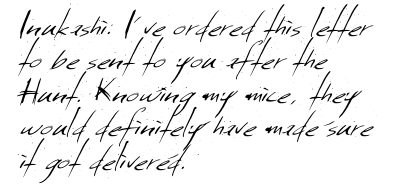
\includegraphics{Images/memo7_nezu.png}\\

The letter began with no~formal opening or seasonal greeting, and read
rather standoffishly.

Doesn't he even know how to write a proper letter? Or does he think I'm
not good enough for a greeting? If that's so then, well, what a rude
prick.

Nevertheless, a letter from Nezumi was unexpected and unusual, and his
eyes were glued to the letter even while he complained. He read, and he
growled.

On the letter were detailed instructions for those left behind in the
West Block. Only after reading the letter did Inukashi finally realize
what meaning was behind the meaningful and suggestive look in Nezumi's
eyes.

I see. This is what you want me to do. What a touching love letter
you've given me.

This guy is just rotten. Not that it's anything new.

He took a deep breath. He had to decide: whether to crush the letter in
his hand and pretend he never saw it, or act on Nezumi's orders.

A short moment of hesitation came and went. Inukashi folded the letter
neatly, and exhaled a long breath.

Apart from instructions for Inukashi, there were also detailed orders
for Rikiga as well. That was the source of Rikiga's discontent.

"The brat thinks he can order me around. Damnit, I feel like that
despicable rat is remote-controlling me. Pisses me off."

"Then you'll ignore it?"

"I can't just do that. Shion's life is on the line."

"The mountain of gold bullion is also on the line."

"Exactly."

Love and greed. These two conditions were often all it took to get most
people moving. For the amount of continuous complaints that streamed
from Rikiga's mouth, he moved surprisingly swiftly and efficiently. He
had brought in a stock of micro-bombs. He had probably had them prepared
a while ago in advance.

He had said he had spent ungodly amounts of money. But if they were
going to get that gold bullion, it was a small sacrifice.

Both Inukashi and Rikiga had accomplished half of Nezumi's orders. Now
there was the other half. This was the critical moment.

"We know for sure that Tsukiyo and the rest are on our side. Isn't that
enough peace of mind for now?" Inukashi voiced his honest thoughts.
Whether it be a human, dog, or little mouse, as long as they weren't
enemies, it was something to be thankful for. He wished Rikiga would
worry about this "strangeness" and "mystery" business later, when they
weren't in such a tight situation.

It's been obvious since, like, a hundred years ago that Nezumi is
someone you just can't figure out, old man.

"Abah, abah, abah." Shionn babbled animatedly.

"Congratulate us, Shionn." Inukashi lifted the tiny body up to the night
sky, where the stars were winking. "Celebrate for us. For our present,
and our future."

"Babhuh." Shionn suddenly lifted his arms, wrapped in a tattered cloth.
He reached straight up as if to indicate at something.

"What?" Inukashi looked up to see the golden city. The Holy City of No.
6, glittering, tore through the inky darkness.

Shionn's tiny fingers were stopped right on that golden light.

"It's No. 6. What about it? Did it catch your eye?"

Shionn wasn't smiling. He wasn't crying, either. With his purple-tinted
eyes opened wide, all he did was stare intently at No. 6.

\hypertarget{index_split_030.htmlux5cux23calibre_pb_54}{}

\protect\hypertarget{index_split_053.html}{}{}

\hypertarget{index_split_053.htmlux5cux23calibre_pb_0}{}

\hypertarget{index_split_053.htmlux5cux23calibre_toc_4}{%
\subsection{CHAPTER 3}\label{index_split_053.htmlux5cux23calibre_toc_4}}

\subsubsection{The Reason Why}

\emph{When people built the public office}

\emph{wasn't the reason why}

\emph{so it could take away their perils}

\emph{and create a bright and peaceful world?}

\emph{But the citizens suffer hardship, and the officials bloat with
riches}

\emph{On the vast earth, not a single one}

\emph{of the citizens can voice their woe}

\emph{So they take to their brushes, and entrust it to song.}

\emph{\\
}

\emph{-Chinese folksong}

Safu let out a scream.

\emph{This is me?}

\emph{Why, why, why...}

"Safu, are you awake? Good morning. How do you feel? Ah, I see all your
cognitive senses have returned to normal. Splendid."

\emph{This is me?}

\emph{No, this isn't me.}

\emph{This isn't me.}

"What are you talking about? Look. You are beautiful. Not only
beautiful―yes, soon you will have both beauty and power in your hands.
And immortal life. Brilliant, is it not?"

\emph{No. No.}

\emph{Help me.}

\emph{Turn me back.}

\emph{Turn me back to who I was.}

"Safu. You cannot let yourself get over-excited. It hurts, doesn't it?
Yes, when your emotions are agitated, it causes pain. Headaches. So,
calm. Calm down. Calm down, and think of the appropriate state you
should be in. Yes... good girl. I will help you. Yes, calm down..."

\emph{Shion...}

\emph{Where is Shion?}

"Forget him. You have been reborn. Forget everything from before.
Everything. No people, no names, or memories are of use to you anymore,
Safu."

\emph{I don't want to forget.}

\emph{I can't forget.}

\emph{I... won't forget.}

"You know, Safu, tomorrow is a festival. A day to celebrate the birth of
this city. A celebratory festival. It's called 'The Holy Celebration'.
You know about it too, I'm sure. You were a former citizen, after all."

\emph{Shion.}

\emph{Shion, where are you?}

"Festivals are utter foolishness. Everyone makes a senseless ruckus and
they don't even realize what they're celebrating for. Foolish, aren't
they? It would be troublesome if they weren't, however. Ha ha ha.... The
real Holy ones are right here. You and I. Shall we give a toast, Safu?
Will you have wine?"

\emph{I will not forget.}

\emph{I will not forget you.}

\emph{I would never be able to forget you.}

"Safu, why are you expressing sadness? I'm planning a very splendid gift
for you, you know. Soon. I will lead you to become an existence everyone
would admire."

\emph{I will keep remembering you.}

\emph{Because this is my own heart.}

\emph{I will not... forget.}

"How troublesome. I thought you would be less of an obstinate child. I'm
a little disappointed, Safu. Very well, then. Soon you will see the
extent of my magnanimity. Then you will prostrate yourself and feel
gratitude for me. See, Safu? Oh, yes, we'll no longer need this name
anymore either. Let us throw it away. A new future is waiting for you,
after all. See? Doesn't it excite you just thinking about it?"

\emph{I will not throw away my soul.}

\emph{I will not lose my memories.}

\emph{My feelings will not be stolen from me.}

\emph{Shion,}

\emph{where...}

"Come on. Come over here."

\emph{Shion, where are you?}

Shion finished talking. He recalled, in as much detail as possible, the
past few years starting from the stormy night when he met Nezumi, to
where he stood today. He knew no amount of talking could tell his whole
story. He didn't have the confidence that he could accurately tell all
that had caused him such turmoil. But he told anyway. Rooting out the
buds of countless emotions that had begun to sprout in his soul, to the
best of his ability, he calmly and objectively told of his own
experiences, what he had seen and heard, the scenery which spread before
his eyes, and the sounds which had travelled through his eardrums. At
least he had meant to.

But still, his voice shook at the end. He couldn't help the plea from
creeping into his tone.

I am weak. So powerless. I can't even repress my emotions with my own
strength.

He clenched his fist.

You knew, Shion. You've known this for a long time. You've been forced
to face the reality of how weak you really are, over and over, before
you came here. What's the use being afraid of your own powerlessness and
ignorance now? You can be ashamed, but you can't be afraid. If you
falter, you won't be able to move forward again. You've come this far.
You can't turn back. You're not that weak.

Shion took a deep breath, and continued his words.

"I want to help Safu. I'll do anything to get her out. That's what I've
come here for. Nezumi brought me here. I can't begin to imagine where
this is, or how I can infiltrate the Correctional Facility from here.
But no matter what, I have to accomplish it. That much I can be certain
of. And... I'm the one that got Nezumi involved. Nezumi risked danger
for me... that's also the truth."

The elder remained silent. They were wrapped in stillness. The silence
was heavy on them, and Shion felt like he could even feel his bones
creaking.

Beside him, Nezumi crouched. He picked up the shirt which had slid from
Shion's hand without him knowing, and handed it back to him.

"Thanks."

Heh.

Nezumi chuckled.

"Your manners don't leave you in this situation either, do they, young
master? Maybe add 'ignorant brat who thinks highly of himself' to that
nickname, while you're at it."

"Me? Think highly of myself?"

"Yeah. I didn't come here for you. Don't flatter yourself too much,
young master."

Before Shion could respond, Nezumi turned aside. His expressionless
profile rejected Shion's gaze and words.

"Rou." The elder didn't respond to Nezumi's call. He remained unmoving,
with his eyes closed. He looked like he was either meditating, or
reciting a prayer in his head.

"Rou, there's nothing false about Shion's story. It's all truth. There
have been casualties in No. 6 from parasite wasps. Shion was spared. But
most of everyone else won't be. They all die strangely―" Here Nezumi
shut his mouth, and glanced at Shion. A shadow of doubt wavered in his
eyes, though only very slightly.

"Rou? Are you listening to me?"

The elder's head nodded slightly. "I am. Your voice projects well, and
reaches the ears of your listeners very clearly."

"Has it reached your heart?"

"Of course."

"Then I want you to answer me. I want you to tell me."

"The fate of No. 6?"

"No, I don't need to ask anyone to find that out. I know what's gonna
happen to it: destruction and extinction. I'll be the one to pull the
trigger."

"Then... what do you wish to ask?"

"What the parasite wasps really are."

Shion let out a soft cry. He looked at Nezumi's profile wide-eyed, and
then shifted his gaze to the elder.

"You are telling me to divulge the truth about the parasite wasps?" the
elder said.

"Yeah."

"Why... do you ask me this?"

"Because you know," Nezumi answered. "I have a feeling you do. I've been
thinking all this time: maybe, just maybe... you know most of everything
I'd want to know." Nezumi exhaled. The stiff angles of his profile gave
way, and doubt shaded his face even more darkly.

"You know, because you were formerly of No. 6, as a citizen... no, as a
creator. Am I wrong?"

This time, no voice escaped Shion's lips. It was caught in his throat.

Creator? This elderly man?

"Is what I'm saying incorrect? Rou."

The elder didn't reply. Nezumi turned his face up at the ceiling. There
was only a pool of dusky gloom. But Nezumi blinked at it rapidly, as if
he were staring at something blinding. Then with an unusually languid
movement, he raised his arm up.

"This." He was holding a square piece of paper between his fingers. He
passed it to the elder. It was a photo, an outdated one that was still
printed on special photo paper.

"The alcoholic old man had it. Your mama's in it too," he said to Shion.
"I took the liberty of borrowing it from his files."

"Oh, that..." It was one of the photos that had been mixed in with the
jumbled contents of several folders. They had been strewn about on the
floor when the two had last visited Rikiga from the directions on
Karan's memo. In the photo were his mother and her friends, several
decades younger. He remembered hearing Rikiga, a former journalist, say
that this was the photo he took the last time he ever entered into No.
6.

Back in those days, No. 6 hadn't been as closed off. There was no law
yet that required a city-issued permit to enter or exit, and it wasn't
like now where anyone who didn't possess a permit was prohibited from
entering under any reason or circumstance. The special gates and alloy
walls also hadn't been completed yet. Rikiga had said that it was still
a time when travelling to and from No. 6's surroundings had been
relatively easy.

"The young woman in the centre is Shion's mother. Her name is Karan."

"Karan."

"You know her, don't you? You're in the picture with her. Or have you
long forgotten her?"

"With her? This man, with my mother?" Shion was surprised. He could tell
his mouth was gaping open. He couldn't help but stare openly at the
snowy-haired elder. He knew how insolent his gaze was, but he could not
avert it.

He knows my mother? To think that this man who had settled in these
underground caves, was called "elder" by the others, was connected to
Karan. It was unbelievable, if nothing else.

Unbelievable, how can that...? For an instant, the surprise hit him so
hard he felt like the core of his brain was tingling.

Since meeting Nezumi, the boundaries of his world had broken. The world
he had lived in before had all but collapsed. Everything was full of
surprises. Things he had believed in, had never had a doubt about,
inverted and showed an opposite face. He experienced this heart-stopping
realization many, many times.

Astonishment, awe, stunned silence, perplexity, and pain. He had
experienced so many emotions and sensations. But he was also being
forced to come to terms with how ignorant he had been before he met
Nezumi, and how he had lived not knowing anything, and not trying to
know.

That was why it hurt. It hurt enough to make him gasp in pain. But even
so―he vowed not to hesitate at being surprised and perplexed.

Shion, in his own way, hoped to see the truth about himself and the
world he lived in. He had also resolved to see through it all. He didn't
hesitate at being surprised or confounded; on the contrary, every time
he was surprised or confounded, he felt a layer peel away, and a new
facet of the world unfold before his eyes. He had even come to revere
the experience.

But this time, he was simply astonished. He fixed his eyes on the elder
with his mouth open. Nezumi's fingers touched his lips. Why were his
fingers always so cold? A feeling most distant from surprise or
perplexity flitted across the back of Shion's mind. Nezumi clicked his
tongue softly.

"Shut it. You have the most unbelievably idiotic expression on your face
right now."

"No way..." Shion whispered. "This is what's unbelievable... Nezumi,
what's going on? How does my mother factor into this? This man and my
mother know each other... what does it mean?"

"How should I know?" Nezumi retorted. "I'm asking you because I don't.
See that photo the alcoholic had: the one standing beside your mama is―"
Nezumi swallowed. "It's Rou."

The photo slid from the elder's fingers. It fluttered to the ground like
a flower petal.

"I was surprised too, when I first saw this photo," Nezumi said. "I
probably had the same kind of expression on my face, though probably not
as idiotic as yours."

Nezumi picked the photo up, and held it out for Shion to see. Shion
leaned forward, and squinted at it. It was a rather aged photograph.
Several young men and women were standing in front of a grey building.
Karan was standing in the middle of them. Her hair was grown out long,
and she was smiling shyly. Her smile still carried a sort of
girlishness. On her right was a tall man with a long face. He was
clutching a lab coat in one hand, and had gentle eyes. Even from the old
photo, Shion could make out the deep intellect that resided in those
eyes.

My godfather. Nezumi had pointed at this man, and said those words. He's
my godfather.

Shion knelt down in front of the elder.

"Please tell me." His voice was raspy. His throat was painfully parched.
"Please tell me the truth. That's all I ask."

The elder's torso swayed slightly. It reminded Shion of swaying silver
grasses. His white hair, which shone dully in the candle light, was
almost like the ears of the silver grasses themselves.

"Knowing the truth, and rescuing your friend: do you think the two are
connected, Shion?" Shion shook his head slowly in answer.

"I don't know." He answered truthfully. He really didn't know.

He had to do anything to rescue Safu even a minute sooner, a second
sooner. But what did he need? Did he need to know the truth about the
parasite wasps, the relationship between his mother and the elder, and
No. 6's future... did he really urgently need to know these things?
Shion didn't have an answer.

He did wish to know. He desperately yearned to know. But the most
important thing right now was to save Safu―was it not?

"I don't know... Maybe my knowing the truth and rescuing Safu are two
completely different things. But..."

"But?"

"But I―or should I say we―we residents of No. 6, including myself, have
been kept away from the truth all this time. We've lived our lives
hidden from the face of reality, the true form it embodies."

"You've just never tried to see it," Nezumi remarked, emotionless. "If
you squinted, you would have seen. If you searched for truth, you would
have found it. But you didn't. You got drunk and giddy on your false
idea of abundance, and settled yourselves into blissful laziness. You
didn't try to look through it to see reality. Your foolishness allowed
No. 6 to burgeon into the monster it is today."

"I'm sure you're right." Shion inhaled. Nezumi was right. But you know
what, Nezumi? In the time I've lived with you, I've been able to touch
the sprouting ears of truth. I touched them with my own hands. That was
my starting point. That's a truth in itself, too.

I started off there, and now, I'm here.

"Safu getting kidnapped, and parasite wasps appearing... No. 6 turning
into a monster, all happened because we've averted our eyes from the
truth this whole time. The crime we've committed is grave; I've realized
that. But that's why I want to know. I want to see true form of the
world, with my very own eyes―"

Shion bit his lip. No, he almost said out loud. It didn't feel right. It
wasn't that he had lied to the elder. But he had decorated his words.
Regret and resignation about the past weren't the only things that lay
behind the reason for his wanting to know the truth.

Curiosity. No, it wasn't such a casual feeling; it was a deep-rooted
desire. It roved in circles deep inside his chest.

It was intrigue towards a world his imagination could not render.
Interest in the unknown. And more than anything... it was the
expectation that he could acquire some piece of knowledge that had to do
with Nezumi.

The part that Nezumi showed him was only a small fragment. In fact,
Nezumi had many faces which Shion could not see through. And he felt it,
painfully, everywhere, every time.

Where did you come from?

Where were you born?

How did you used to live until that stormy night when we met?

What have you thought about, believed, and rejected in your life up
until then?

And there's the promise of telling me your real name, which you haven't
fulfilled yet.

His soul was stirring restlessly. It stirred from wanting to know, and
not for anyone else but himself. But he had put on an act. He had
pretended to be the friend, the innocent youth who longed to know the
truth.

His heart and words turned away from each other. How beautiful and
rational were the words that spilled from his mouth. They were rational
and beautiful to the point of sounding fake. His own words deceived his
heart.

He bit his lip. He chewed on it hard.

Can I only speak in these kinds of terms?

Why can't I speak like Nezumi? I can only use empty, superficial words.
Why do I keep putting on an act? Why do I still speak, when I'm not even
prepared to reveal my true self?

Even though I've lived by his side for months...

He had directed his gaze at Nezumi without even thinking. There was no
way he couldn't have noticed the decoration in Shion's words, but
Nezumi's profile showed no hint of disdain, scorn, or pity. He had
lowered his chin slightly, and was staring off into the dark void.

Nezumi never toyed with his words.

Safu was the same.

Like a flash of lightning in the night sky, an idea sparked in his mind.
Safu had never manipulated her words. At least, any words she had
directed at Shion were true. He had received her straight and earnest
words numerous times.

He realized he ought to be ashamed of himself. Both in the face of
Nezumi and Safu, he ought to be ashamed of himself.

"I... want to know." He squeezed out each word painstakingly. "There are
too many things I don't know. That's why... I want to find out. That's
it."

The elder's body swayed once again. "Just because you know, it does not
mean it will make you happy. You may end up wishing you had never known
at all. Such a reality may be waiting for you, Shion."

"I'm prepared for it." He would rather suffer from the knowledge than
being blissfully ignorant. He preferred the pain and hardship of truth
rather than fake happiness. With this as his fuel, he could move
forward. He couldn't keep leaning on this illusion, which didn't even
serve as a foothold.

He clutched his chest. He confirmed his feelings.

There was no doubt about it. My feelings are here within me. I am not
deceiving anyone.

"I'm prepared. At least, I think I can prepare myself. Though―I can't
say for sure that I won't regret it... I'll probably regret it a number
of times... but I feel like it would be much better than going without
knowing. That much I feel is true... so, ah, I..." As soon as he tried
to speak in earnest, his tongue refused to co-operate. His words refused
to run smoothly as they had just moments before.

Earnest words were heavy things.

They bore the weight of the speaker's beliefs, emotions, and honest
feelings.

The elder suddenly smiled. At least to Shion, it seemed like he did. The
elder let his momentary smile fade, and slowly lowered his eyelids. He
fell silent.

"Rou, why are you silent?" Nezumi asked harshly in impatience. "Rou!"

"Elyurias." The elder's lips moved, and a whisper, like a breath,
escaped. It was a word Shion couldn't understand.

"Elyurias?" Nezumi furrowed his brow. Apparently, he hadn't understood
either.

"That is the name."

"Whose?"

"Hers."

"Her?"

"Nezumi, your eyes."

"Huh?"

"Close your eyes. Shion, you also."

Shion and Nezumi looked at each other. The elder's voice was low and
placid, and carried no hint of a command. But he found himself obeying
it nevertheless. He felt like he had let himself go limp on the gentle
flow of a river, and he was being born to the sea. Shion closed his
eyes.

"Elyurias," the elder whispered again. "She was a great sovereign. She
was a rare existence."

Elyurias...

Nezumi sucked in a breath from beside Shion.

"Looking back, it seems a thing of the distant past," the elder
continued. "It was still a time when this land... yes, this land was
still without walls. Instead of walls, there was a lush green forest.
There were lakes, marshes, and grassy plains. Myriad things intertwined
and maintained a harmony. A paradise... it may have been the last
remaining paradise on this planet. A paradise that had escaped the
destruction of humankind. A land of miracles. A place that could nurture
life and put death to rest. She resided there. She really existed. I was
the one who found her."

The elder's voice dropped even lower.

"Ah, no... that is an arrogant way to put it. I did not find her. I met
her. We met by chance... as if God had drawn us together. Elyurias―she
was a great sovereign. She would likely be one to this day. She still
reigns."

"Elyurias." Shion said the name under his breath, imitating the elder.
Elyurias. It was a sound unfamiliar to his ear and tongue. He couldn't
imagine what kind of appearance or voice a person with that name would
have. Not to mention someone who was a "great sovereign"... Shion cocked
his head in disbelief. It sounded too grandiose, too phony. He sensed
domination. Had a kingdom existed here in the past? Just like how No. 6
dominated this land now, this sovereign called Elyurias had governed
all...

'She', the elder had said. Then that would make her a queen. A paradise
governed by a queen? That sounds like a cheap drama. I find it hard to
believe.

The air shifted just slightly. He heard a hoarse groan. As Shion lifted
his eyelids, the first thing that jumped into his vision was Nezumi
covering his face with his hands. He was about to buckle to his knees.

"Nezumi!" Nezumi collapsed into his outstretched arms. Shion felt the
heat and weight of his body. A low groan trickled through Nezumi's
fingers. It's the same. It's the same as last time.

They had been talking about parasite wasps in their basement dwelling.
It was just when their conversation had moved from emergent viruses to
the mystery behind the parasite wasps. Nezumi had suddenly collapsed.

They had been drinking hot water. Shion remembered how Nezumi's cup had
slid out of his hand and bounced on a stack of books before rolling
across the floor.

"Nezumi―relax. Can you hear me?" Shion knelt down, supporting the boy's
body with his arms. If it was the same as last time, then there was no
need to panic. Nezumi had recovered just fine last time. If this time
was the same...~

"Ow!" A set of fingers dug fiercely into Shion's arm. Nezumi gasped, his
chest rising and falling. The tremor of his fingertips agitated Shion's
worry even more.

"Water," Shion muttered, glancing all around. No one moved. "Please,
give me water. Anyone."

"Will he die?" a voice asked from behind. It was flat and cold. It
belonged to Sasori, the sand-coloured man. He had drawn right up behind
them without Shion noticing.

"Will he die? Then there is no need to bring water." Contempt wafted
into Sasori's tone. "There is no need to give anything to the dying.
Furthermore, he is one who has once left. No need. At all."

Shion turned around. He looked up at the man who had concluded the
discussion with such terse words. No need.

"Bring it," Shion commanded. As far as he could remember, he had never
given an order to someone in such an oppressive manner. But the words
didn't feel strange leaving his mouth.

"Bring water to me. Quickly."

Sasori shifted uneasily. The rims of his widened eyes twitched. A single
bead of sweat rolled down from a corner of his eye.

"Here." A wooden bowl was handed to him. It was about half-full with
water. A small, thin child was holding it out as if it were an offering.
"Mother told me to―take this."

"Thank you." Shion accepted the bowl from him. The child spun around,
and trotted away into the darkness.

Cheep-cheep.

A small mouse scurried up onto Shion's shoulder. It stared at Shion's
hands, twitching its nose.

"Nezumi... drink this." Supporting Nezumi's body with one arm, Shion
slowly tipped the water into his mouth. Nezumi's throat contracted. He
took a gulp.

"Nezumi, can you hear me?"

His eyelids lifted, and a pair of grey eyes peeked from underneath.
Shion thought they were beautiful. They were the colour of the sky at
the coming of morning. They absorbed light, yet released it softly at
the same time.

They were beautiful like the dawning sky.

A lightening sky at morning conjoined somewhere with the hope of life.
It was a glow that lauded people who had resolved to live, or at least
try to live, through today. That was why it was beautiful.

I've gotten so much hope from the beauty of these eyes.

Shion clicked his tongue at himself. Idiot, now's not the time to be
admiring him.

"―Shion."

"Are you awake? Drink the water slowly―there―all of it. Then take a deep
breath."

Nezumi obediently did as he was told. He drained the water, took a deep
breath, and exhaled.

"You alright?"

"Somewhat."

"Does you head hurt? Any nausea, or palpitation―"

"Ten."

"Huh?"

"Three plus seven is ten. And since I'm at it already, twenty-one."

"Oh... three times seven." So Nezumi had remembered the questions Shion
had asked when he'd woken up last time. Shion stifled a chuckle. Yes,
reality was brutal and cruel. The past few hours had been filled with
human despair, death, and screams. It was dyed through with the colour
of terror, futility, and intense regret. But there had also been many
heartwarming moments, moments where his pulse had quickened and his
spirits had soared. Memories with Nezumi were always like that. They
always brought excitement and warmth to his heart.

Memories?

Shion straightened his back, and put more strength into his arms. Why
did I just think 'memories', like he was someone of the past? Nezumi
mumbled in Shion's arms.

"I heard the wind."

"Wind?"

"The wind was singing. I heard its song." Nezumi raised himself. "I've
heard it before. But this time it was... it was clearer. It was a gentle
melody..."

"What kind of song was it?"

"It was..."

"Can you sing it?"

"Me? Hm... well. I wonder if I can."

"Let me hear it."

Nezumi blinked, and his lips moved. A song with a lilting melody poured
forth.

\emph{The wind steals the soul away, humans thieve the heart}

\emph{O earth, wind, and rain; O heavens, O light}

\emph{Keep everything here}

\emph{Keep everything here, and}

\emph{Live in this place}

\emph{O soul, my heart, O love, my feelings true}

\emph{Return home here}

\emph{And stay}

The little mouse grew still on Shion's shoulder. It stopped moving as if
rooted to the spot, and quieted its breath. Humans all around did the
same. The people hidden in the darkness were also frozen in enthralment.
Their eyes were closed, and their bodies were lent fully to the song.
Everything grew still. It felt like even time had stopped. Nezumi's
voice, and his song, seemed to soak into them, enveloping them, rocking
them, and making them feel as if their bodies and souls were floating.

\emph{The wind steals the soul away, humans thieve the heart}

\emph{But here I will stay}

\emph{to keep singing}

\emph{Please}

\emph{Deliver my song}

\emph{Please}

\emph{Accept my song}

The song ceased, and someone let out a gentle sigh. He was not the only
one. Here and there in the darkness, soft sighs could be heard. Nezumi
slowly shook his head.

"I feel like I've heard it before. Like I've heard it over and over,
since a long time ago. Someone's taught me this song before."

Shion lifted his head and posed a question at the seated elder.

"Is this song somehow related with Elyurias?"

"Do you think so, child?"

"Yes." The moment he had blurted the answer, he felt certain. Nezumi and
Elyurias were connected. The elder narrowed his eyes, and his gaze
wandered in the air.

"It has been a long time since I heard it. I was convinced it had long
disappeared from this land. I see―there still remains a person who can
sing."

"The wind sings." Nezumi wiped his wet lips with the back of his hand.
"Or maybe someone's singing in the wind. And I... hear it. I've come to
hear it."

The elder nodded. "Since when?"

"A little while ago. Yeah―a little while before the Hunt. This is the
third time. When it happens, my consciousness fades, like a stage in a
blackout... and then green scenery appears... and then..."

Nezumi's eyes turned to Shion. His gaze wavered. Shion remembered that
stormy night, the night he and Nezumi had met. The boy had appeared
before him, soaked and blood-stained. He was so fragile, Shion had felt
like he would make the boy fall apart just by touching him. Drawn to
that fragility, and those vibrant eyes which were so much the opposite,
Shion had extended his hand.

"I'll treat your wound." Those words had escaped his lips without a
shadow of doubt, without resistance. He had felt like he had to do
something. He had felt like it was his duty to protect this boy. He had
never felt this protective of anyone, neither before nor after this
incident.

A sharp, vivid moment. One that had burned an imprint into his life.
Every time he recalled it, his heart quickened.

The fragility that had stirred Shion's protective instinct―the same
fragility that had been completely wiped clean when they reunited four
years later―returned into those eyes again.

His heart quickened.

"I don't know," Nezumi continued. "I was still young, and I was wading
through the grass. And I could see... the sky."

"Right."

"An ultramarine sky. It was a really beautiful blue. And wings
buzzing... and a song. I couldn't tell whether it was man's or woman's
voice. It was a strange voice. It almost sounded like the wind, crossing
the plains, or crawling across the ground, or showering down from the
heavens. I... I was always just standing there... listening to that
song..."

A song of the wind which crawled across the ground, and showered from
above. Maybe...

"Was it a song of offering?" Shion said. It was mostly instinct. The
spark of an idea turned into words, and spilled from his lips. "A song
offered to Elyurias... either to praise or appease her... am I right?"

The elder's chest swelled and deflated. It looked like he was taking
several deep breaths. Is he agitated? Confused?

"Sasori," the elder called. The sand-coloured man materialized like a
blot in the darkness. "Provide these two with food and rest."

"Rou―"

"They will probably not have much time to rest... but that cannot be
helped. Provide them whatever they wish for, to the best of your
abilities."

"Why?" Sasori yelled angrily. "Why do you help them? Nezumi is one who
has once left this place. He left, vowing never to return again. He was
forbidden to return, was he not?"

"Yes."

"But he did return. Bringing a demon with him, nonetheless. Rou, can you
not understand? He is evil itself. He brings calamity and destruction."
Sasori's finger pointed squarely at Shion.

"Did you see his eyes just now? Those are the eyes of evil. The eyes of
wicked darkness. Nezumi is being puppeted by this demon."

"Now you listen." Shion was now feeling more than cross. "You've been
repeating yourself all this time. I only glared at you a little, and
you're making me sound like I'm some monster. Kind of rude, don't you
th―"

Sasori cut Shion off by shaking his head. His face contorted, as if
every word Shion uttered was a curse.

"The very picture of a monster. Rou, I am fine with Nezumi. If you
command me, I shall obey. I will provide him rest and food. But I cannot
do that for him. If we do not kill him now, then he will bring
misfortune upon us. He may obliterate us entirely."

"Sasori." Nezumi stood up. "Sometimes poison and medicine can come from
the same plant. Sometimes you can't tell if it's going to be poison or
medicine until you drink it. Right?"

"...What is your point?"

"There's no need to reveal Shion's so-called true identity, whether he's
a demon or not. His identity doesn't matter. Right now, all I care about
is that he's kept alive. That's all."

"Why?"

Nezumi's fingers grasped a handful of Shion's hair.

"Inside this head, Sasori, is information about the inner structure of
the Correctional Facility. The most up-to-date stuff. I can bet it's
probably as accurate as computer data. I wouldn't be able to destroy the
Correctional Facility without it."

"Destroy the Correctional Facility―" Shock spread across Sasori's face.
Just for an instant, it the expression made the sand-coloured man
actually look human. This man had shown the same reaction to Nezumi's
words as Rikiga and Inukashi did. Ah, I see, Shion thought.

His skin and eyes were a strange colour, but those were the only
differences. This man was made of flesh. Blood coursed through his body,
and he gave off heat. He would feel pain if he was wounded, and he had
both emotions and intelligence. He was a human, just the same. Skin and
eye colour were such small differences, they didn't even seem to count.

"Surely you are not really thinking of doing that?" he said in
disbelief.

"I am," Nezumi said promptly. "In fact, that's probably all I've been
thinking about. The Correctional Facility isn't just a prison. It's also
a research organization that's connected to the core of No. 6. If we
destroy it, it'll put a crack right in No. 6 itself, for sure. We're
going to use that crack as a foothold to throw No. 6 into its grave. And
to do that, I need Shion. I told you before, Sasori, I won't let you
kill him that easily."

The elder opened his mouth before Sasori could.

"There may already be a crack appearing."

"What? What do you mean?"

"No. 6 may disintegrate even before you strike a blow, because of
Elyurias."

"Rou!" Nezumi barked irritably. "Speak in a way I can understand. So far
you haven't clarified a single thing."

"Nezumi, perhaps it is fate that you have returned with Shion. Perhaps
it had already been decided beforehand."

"Beforehand?" Nezumi retorted. "Who the hell can decide how I'm going to
live? I'd like to see anyone try. I'll never bow down to cheap words
like God or Fate. That's enough, Rou. No more word-play. Stop your
mysterious nonsense and answer my question. You were involved in the
birth of No. 6, correct?"

"Yes."

"How?"

"Be seated. You too, Shion. Be at peace. I will give you water. You are
probably thirsty." Before the elder even finished his words, a pair of
slightly bigger bowls were being handed to them. They were filled with
clear water.

Shion felt a powerful thirst return to him.

He hadn't realized how badly he had wanted water. He felt like all the
moisture had been wrung out of him in the numerous experiences leading
up until now. He was so thirsty, he felt like his throat was chafing.
When he had fed Nezumi water earlier, he had not wanted any for himself.
He had completely forgotten his thirst. But now it was like his parched
state was a reaction to that; he felt like he was burning up.

"Water―" Shion held the bowl in both hands and greedily gulped it down.
It was cold and delicious, like the water that Nezumi had fed him over
and over during his battle with the wasp―the water that ran near
Inukashi's ruins. It had the same taste. It was delicious, and it
quenched him.

He drained it in a single draught. More water was poured into his empty
bowl. Shion was so grateful he felt he could cry.

"Good, isn't it?"

Shion found himself nodding vigorously in answer to Nezumi's question.
It was too good to put into words.

"There's an underground lake here. Lots of minerals. ―Geez, you must
have been thirsty."

Shion finally stopped to take a breath after he had had several bowls of
water. The elder must have been waiting for him, for now he opened his
mouth to speak.

"This will take a rather long time. I had intended not to tell anyone
for my whole life... but I must tell it now. However, before that...
Nezumi."

Nezumi lifted his chin.

"There is a path leading to the Correctional Facility, but it is only
connected partway. The Facility has built a door from their side sealing
the way off. It has not been opened for decades."

"I know."

"There is no other way into the Correctional Facility unless you open
it. You know that too, I presume?"

"Naturally."

"It is impossible to open it from this side. Nor will it ever open from
the Facility's side. It absolutely will not happen."

"The thing with doors―" a wan smile spread across Nezumi's lips, "is
that you don't just wait for them to open politely by themselves. You
force them open."

"Have you a plan?"

"I'm not unprepared."

"I would not have expected you to act without some strategy. But I
cannot imagine how you would open the door."

"Shion." Nezumi crouched down, and put a firm hand on Shion's shoulder.
The startled mouse hastily hopped down out of his way. "The door we're
talking about: it's the only point on the map that connects the blank
space underground to ground-level. You know where it is, right?"

"Yeah." The floorplan appeared in his mind, the one of the Correctional
Facility that Nezumi had commanded Shion to memorize as if his life
depended on it.

"It's in location po1-z22. From the Facility's side, it was labelled
Point X."

"You remember the energy circuits which were connected to that point
too, right?"

"Yeah. It was a single circuit, an old system. There are no auxiliary
circuits."

"The unopenable door doesn't need a carefully-crafted backup system,"
Nezumi said. "Efficiency is paramount. Remove everything else that isn't
absolutely necessary. Both people and machinery." He chuckled. "Sounds
like something they would think of. But this is where it works to our
advantage."

Nezumi snapped his fingers.

"The unopenable door opens. We'll pry it open. Rou, we'll fight our own
battle. You have nothing to worry about."

"Only death is waiting."

"For us?"

"For many people. Many more people will likely die, more than you can
imagine. Perhaps you are the only ones who can stop that. Nezumi, fate
does exist. Fate has brought you together, and you are here because of
fate. It was fate that Elyurias and I met. Let us begin with that story
first. Listen well, and make haste, or else it will be too late. You
must hurry...."

Then the elder began to speak. It was a story of No. 6.

Shion and Nezumi huddled together and grew still, like children
listening to their grandfather tell a tale of the past. Only their ears
strained hard to listen.

It was a story of No. 6.

A tale of destruction and creation.

\hypertarget{index_split_053.htmlux5cux23calibre_pb_80}{}

\protect\hypertarget{index_split_078.html}{}{}

\hypertarget{index_split_078.htmlux5cux23calibre_pb_0}{}

\hypertarget{index_split_078.htmlux5cux23calibre_toc_5}{%
\subsection{CHAPTER 4}\label{index_split_078.htmlux5cux23calibre_toc_5}}

\subsubsection{Leave Every Hope}

\emph{Through me is the way into the woeful city;}

\emph{through me is the way into eternal woe;}

\emph{through me is the way among the lost people.}

\emph{\\
}

\emph{Justice moved my lofty maker:}

\emph{the divine Power, the supreme Wisdom}

\emph{and the primal Love made me.}

\emph{\\
}

\emph{Before me were no things created, unless eternal, and I eternal
last.}

\emph{Leave every hope, ye who enter!}

\emph{- Dante, The Divine Comedy Vol 1: The Inferno, Canto III~}

It began suddenly. No one would have been able to predict it.

It began suddenly, and amidst the crowd that had gathered in the square.
It began as when gas erupts after being compressed for a long time
underground.

\textbf{The Holy Celebration Day, 2017.}

\textbf{12:15 pm}

\textbf{Front Square, City Hall (also known as The Moondrop)}

The wind blew icily and nipped at the skin, but the sun was bright. The
sky was clear, and was dyed a brilliant blue, appropriate for the
festivities. The hearts of the people were buoyant. They waved flags,
and all praised the Holy City.

"Our mighty No. 6."

The square in front of the city hall where the ceremonies were to be
held was bursting with people.

"It's hot," complained a woman in the stuffy crowd. She was young and
slender. "I feel like I'm going to suffocate, there's so many people."

"So true," her friend agreed beside her. She was short, with black hair.
She sighed as she dabbed the sweat off her nose. "Isn't it horrible, how
there's barely even space to walk? How disgusting to sweat in the
winter. I feel all sticky."

"Really, I don't believe it. We dressed up for nothing."

"I know."

Both had barely any experience of sweating. They had always lived in
places where the temperature and humidity were adjusted just so for
maximum comfort. They couldn't stand the sweat that streamed under their
arms and down their backs. They found the heat of the jostling crowd
exceedingly unpleasant.

The black-haired woman pouted her painted lips.

"My supervisor said I absolutely had to participate in the ceremonies.
If I didn't, I would get my salary cut."

"Me too. Boss' orders. He said it's mandatory that I show up. If it
wasn't, I definitely wouldn't be here."

"They'd know from your ID card if you didn't show up, wouldn't they? The
gates scan your citizenship number when you pass through them... and I
heard they notify your workplace afterwards."

The slender woman nodded gravely, and furrowed her brow. A bead of sweat
rolled down her cheek.

Oh, how unpleasant. I wish I could take a shower and freshen up.

The black-haired woman continued loosing her stream of complaints.

"My younger sister is still a student, but she told me all of them have
to meet at school, and they get bussed over here."

"Really? They didn't have anything like that in our day, did they?"

"No. I heard it's just started this year. They want to confirm your
loyalty level to the city. My sister was complaining that if you don't
participate, you get negative points for your Activities column. You get
placed in Rank D. That means you wouldn't be able to get further
schooling, or land a job. I thought it was a bit harsh, don't you think
so?"

"It is. They're practically forcing us. And speaking of which―it's a bit
much these days, isn't it? Everywhere you go lately, it's loyalty-level
this, loyalty-level that. I kind of find it weird―"

The slender woman was interrupted suddenly as somebody grabbed her by
the arm. White shirt, grey pants. He was a nondescript middle-aged man
with a strong build.

"Um, what―?" the woman began.

"What were you talking about just now?"

"Excuse me?"

"What were you two talking about just now?"

The two women looked at each other. Their hearts quickened. "W-We were
only talking about... you know, how hot it was... stuff like that..."

"Is that so? It rather sounded to me like you were expressing some
dissent, discontent towards the city. Am I wrong?" The man's narrow eyes
glinted. His words were courteous, but the light in his eyes was sharp
and fierce. It made the women cower. Fear pierced through their bodies.

The Security Bureau.

"N-No!" they protested. "Discontent―no―never, we would never say that.
We would never think of that. Not us, we would never..." The
black-haired woman clasped her trembling fingers to her breast. Tears
welled up in her eyes. Help me. Mom, Dad. Help me.

"No matter. Will you kindly let me escort you two? We will have plenty
of time to hear your story later."

"How can you... that's not.. no..." Unable to bear it any longer, the
black-haired woman began to cry. The slender woman was also shaking.

"Kindly let us escort you." Another man in similar clothing materialized
and grabbed the woman's arm. His fingers were shockingly cold.

No―that's not fair, we were only having a conversation. We were only
saying our thoughts out loud.

She was so stunned by the incident, no tears came. She could not cry
like her friend. The slender woman only trembled.

"Come, then." The man's eyes flashed incisively.

I'm scared. I'm so scared. Help me, Mom, Dad.

―Mmgh.

There was a muffled groan. It had trickled from the man's mouth. His
eyes were bulging, wide open, and his mouth was opening and closing like
a fish. No voice came out. Only his lips moved. His hands tore at his
neck. His face began to discolour into a dark shade.

"Wh-What's the matter?"

The man with the cold fingers reached out towards her.

Ahhhh!!!

The woman screamed. She felt like her shriek would tear her throat
apart. The black-haired woman had started screaming at almost the same
time.

"Oh God!"

The man stopped moving. He stiffened, his eyes and mouth still open.
They could see inside his mouth.

Plunk.

Something fell to the cobblestone with a soft sound. Something small and
white...

Teeth.

All the man's teeth were falling out of his mouth, one after another.
His hair was also falling out. Clumps of it turned white and scattered
all around. The man's eyes rolled back into his head as he fell
face-forward onto the ground. His body convulsed. A black stain spread
from his neck. It swelled into a bump, and then―

An incomparably stronger wave of fear came crashing down onto her. She
felt like she would go insane. Perhaps she was insane already. Perhaps
she had gone mad, and that was why she was seeing something that wasn't
supposed to exist. She had no other choice but to scream. She had to
raise her voice, and release her terror somehow. If not, her body would
swell and burst. She would shatter.

The woman breathed in.

Ahhhh!

Eeeeek!

Before the woman could open her mouth, shrieks and bellows welled up
from the rest of the crowd. Here and there, they rose and burst. Voices
of men, shrill screams of women, yells of young people, the clamouring
of the elderly―everything writhed, mingled and twisted around.

"Nooo!!" The black-haired woman was frantically flapping her hands and
feet. She looked like she was doing a disturbing dance.
"Someone―someone's there. Inside me. Help―help me―!" Her teeth fell out
as she opened her mouth to scream.

Plunk, plunk, plunk.

A stain was spreading from the black-haired woman's neck.

"It's poison!" someone was saying. "Run! We've been poisoned."

She heard another voice. It was saying, "we're all gonna die."

It's poison. Run. We're all gonna die. It's poison. Run. We're all gonna
die.

The woman stepped over the fallen man, and tried to break into a run.
But before she did, she saw something glitter suddenly before her eyes.
A bug? Someone shoved at her back. A fat woman tumbled and fell close
by. A mass of bodies stampeded over her ruthlessly.

This is Hell. I have to get out of here―quickly―right away.
Unconsciously pressing a hand to her own neck, the woman leapt over the
bodies strewn on the ground, and broke into a desperate sprint.

The Holy Celebration Day, 2017.

7:02 am - Lost Town

Karan was baking pastries. Cravats, in fact. She twisted the dough,
which had powdered almonds in it, into the shape of a necktie. She fried
it, flavoured it with orange curacao, and sprinkled it with icing sugar
as a finishing touch.

"It looks delicious," Lili said as she swallowed hungrily.

"And it is. Let me set aside ones I won't put out for the shop, and
we'll eat them together with some tea. Or would you prefer some warm
milk with that, Lili?"

"I want cold milk. I like cold milk better."

"Alright, we'll do that. Some nice iced milk, but not too much, or else
it'll give you a tummy-ache. But remember Lili, before that―"

"I have to help with the store, right?" she finished. "I'm gonna do a
really good job. I love being able to help with your store, ma'am. It's
exciting."

"Today's the Holy Celebration, so it'll be very busy."

"I know. First I say 'hello and welcome' right, and then I put the rolls
and muffins in the bag."

"Mm-hmm. And make sure to tell them, 'please feel free to use the trays
on the table by the entrance. You can put your items on them.' And if
the customers are children, or can't use their hands or legs, ask them,
'may I get that for you?'"

"'Hello, and welcome! Please feel free to use the... the..."

"Trays on the table, by the entrance."

"Trays on the table by the entrance. You can put your items on them. May
I get that for you?"

"Brilliant, Lili! That's the spirit. And don't forget to smile."

Lili's nostrils flared appreciatively. "It's easy to smile when it
smells so good. My cheeks just melt, like this." As she cupped her own
cheeks, a shadow flitted across Lili's eyes. Her tone dropped slightly
too.

"Ma'am?"

"Yes, darling."

"Can I take some of these pastries back to Daddy?"

"Of course. I'll leave some for both your Mommy and Daddy―why, Lili,
what's wrong? Has something happened to Renka?"

Karan had heard that Lili's mother Renka was pregnant with her second
child. Perhaps something had happened. Residents of the elite
residential area of Chronos would be promised thorough and meticulous
aid and treatment from specialized medical staff, from conception to
birth. However, a Lost Town resident could only dream of receiving
medical care at the level of Chronos residents. The mortality rates of
invalids, the elderly, and children were manyfold compared to Chronos.

Karan was not discontented with her life in Lost Town. But numerous
times, she found herself forced to face the fact that they were at the
very bottom of the rigid hierarchy which the city had created.

She felt her spine freeze.

She felt a chill not from the realization that they were at the bottom,
but at the very reality that people were dominating over other people
and reigning over them in this way. She also felt a chill at herself,
for not realizing this sooner.

Oh, how careless she had been.

Lili shook her head. Her fine, flaxen hair swished.

"It's not my Mommy. It's about Daddy."

"Getsuyaku-san? Has something happened to him?"

"He had to go to work, even though it's the Holy Celebration Day."

The Holy Celebration was one of No. 6's most revered holidays. Education
institutions and government organizations were closed as a matter of
course, as well as most city shops and offices. The majority of citizens
gathered in the square in front of city hall to listen raptly to the
mayor's speech, and to celebrate the birth and proliferation of No. 6.
Participation had been moving more toward mandatory since last year. By
making citizens pass through gates into the square, the city could tell
instantly if they did or did not participate in the ceremonies. Any
citizen who did not have a valid reason for not participating that fit
the criteria laid out by the authorities were investigated in detail.
Rumour said they were more like interrogations.

Karan felt that this city was becoming more suffocating by the day. But
still, many citizens participated in the festivities not because they
were forced, but because they wanted to. They gathered of their own
will, and waved their gold-embroidered flags of white cloth. Of their
own will -- was this really so?

"Ma'am, the pastry." Lili was blinking. Karan realized she had been
clenching a cravat in her fist.

"Oh, dear, I've let one go to waste. So," she hastily resumed,
"Getsuyaku-san couldn't take the day off?"

"Nope..."

The Holy Celebration was a large event, but there were still many people
who went to work as usual, or else had no other choice but to go to
work. Karan was one of them. She could not live if she didn't work.
Cakes and sweet buns sold exceedingly well on celebratory days. On these
days "the cash came rolling in", to be vulgar about it. Karan had
planned to use this reason not to participate in the ceremonies this
year. On her Application for Non-Participation, which had to be
submitted beforehand, she had to fill in her job description, monthly
profits, and the predicted earnings if she opened her shop during the
holiday. She was also required to submit it in person to the reception
counter of the city. Although it was extra hassle, and although it would
have been much easier to just close her shop and participate, Karan
chose not to.

I can't let myself be pushed along down the easier path.

She had always let herself be pushed into making the easier choice. She
had gotten out of practice of swimming against the current. She had let
her heart go numb, and been swallowed all too easily in the flow. Hadn't
she learned the hard way what the result of that had been?

Her son had been snatched away.

Her son's best friend had been snatched away.

Her most important things had been snatched from her suddenly and
unfairly. She would not let herself be washed away anymore. She had to
dig her heels in, or else she would be ashamed to look Shion or Safu in
the eye again. She would not be able to throw her arms around them
unreservedly when they came home. That was the last thing she wanted to
lose.

"Lili, are you lonely because your Daddy's not here? But I guess we
can't help it if it's his job, huh."

"No," Lili protested. She shook her head again. "Mommy already said we
can't help it. But that's not it. I'm not lonely because of Daddy. I get
to help you with your shop, ma'am, and it's exciting. All my friends
were jealous when I told them I got to work at a bakery―so I'm not
lonely, I'm just―I'm... I'm worried."

"About your father?"

Lili nodded.

"Why? Has something happened that's making you worry, Lili?"

"Not really," she said hesitantly. "Daddy always gives me a kiss on the
cheek before going to work. He said it makes him feel all happy inside.
He said it's kind of like a good-luck charm."

"My, isn't that nice of him."

"Yeah. He's the best. But today, he forgot. He went to work without
kissing me. He left by himself, while Mommy and me were talking in the
kitchen... he didn't even say he was leaving. He just left."

"Maybe he was busy."

"I dunno. But he didn't eat much breakfast either. Just half a slice of
bread and coffee. He was sighing, too. Like this." Lili slumped her
shoulders, and let out a huff of air.

Karan felt an outpouring of love for her.

Lili was concerned about her father, in her own way. 'Maybe he's
troubled about something, maybe he's tired'―she noticed these little
changes in her stepfather, her mother's second spouse, with a sharp eye.
And she was concerned about him. Lili had the experience of losing her
father right before her eyes at a young age. Did this kindness of hers
come from this experience?

"Lili..." Karan felt love for this tiny little soul. She crouched down
at eye-level to Lili, and stroked her flaxen hair. "Keep smiling. Your
smile is my good-luck charm. It makes me sad when I see you with that
frown, Lili."

"Ma'am... Daddy didn't kiss me today, but that's okay, right? God will
protect Daddy, won't He?"

"Of course. I know: why don't you give your Daddy a kiss this time when
he comes home, Lili?"

"Sure, I'll do that."

"Alright, let's open the store, shall we? Can you line the cravats on
the tray and put them out on the rack?"

Cheep-cheep. She heard squeaking.

"Mr. Mouse! You're still here?" Lili chirped happily. A brown mouse was
twitching its nose from underneath the table. It placed its front paws
together, and bobbed its head up and down. Karan realized quickly that
it was a farewell gesture.

"You're going back to your master, then?" And back to my son? Karan
broke off a piece from the pastry she had crushed in her fist earlier,
and placed it in front of the mouse. The mouse picked it up in its front
paws, and began to nibble at it without hesitation.

"Ma'am, look, the pastry and Mr. Mouse are the same colour."

"Oh. Come to think of it, they are. You have the same colour of fur as a
cravat."

Cheep cheep cheep. The mouse raised its face and fixed its gaze on
Karan. It had beady grape-coloured eyes.

"Cravat... is that your name? Cravat?"

Cheep-cheep. The mouse squeaked back as if to say, 'yes it is'.

"Cravat. What a nice name. Goodbye, then, Cravat. Please tell your
master that I'm thankful. That his words give me so much support... I'm
very, very thankful. Please tell him that." And if you can, please tell
Shion too. That I'm waiting―that Mom will always be waiting, and she'll
never give up. So tell him to come home alive.

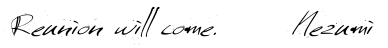
\includegraphics{Images/memo7.png}\\

The short letter she had received from Nezumi. How much courage those
words had given her.

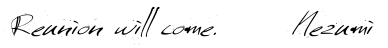
\includegraphics{Images/memo7.png}\\

What a firm and valorous message it was. It had supported her crumbling
heart all this time. Nezumi, would I have the chance to embrace you?
Would I be able to take you in my arms along with Shion? I could keep
waiting, couldn't I, and believe that I can someday?

Cravat finished his last morsel, touched his front paws together, and
bobbed his head. Then he scurried off into a corner of the room, and
quickly disappeared out of Karan's sight.

"There he goes." Lili frowned. "Is he gone forever?"

"No, we'll see him again. Certainly some other day. Right, let's open
the shop. It'll get busy, and I'm counting on you, Lili."

"Yes, Ms. Shopkeeper! Leave it to me." Lili swept into a theatrical bow.
Karan laughed as she opened the door of her shop. She could see the sky.
Its clear blue made her eyes water. The wind was freezing, but it looked
like it would be a sunny day. It looks like the weather will be great―

She felt a chill. Goosebumps formed on her skin.

What? What is it?

She clasped her hands together instinctively. It was cold. She felt like
her whole body was growing cold from the inside. It was only for a split
second, but she felt her face tense, and her hands and feet turn rigid.
The hairs on her body stood on end.

She felt her skin bristle. Again, and again. Something was closing in on
her, something she couldn't see.

A crowd of chattering people passed alongside her, city flags in hand.
They were participating in the walking rally from the Lost Town gates to
city hall. She saw several familiar faces. There were those who nodded
at Karan in acknowledgement; those who gazed at Karan curiously; those
who paused in their step to smell the aroma of fried pastries which was
wafting out onto the street. There was a father holding hands with his
child; young couples; an old woman with a hat perched upon her snowy
head.

They would walk to city hall, and from there take part in the
ceremonies. Midway through the route, all participants were supposedly
going to receive boxed lunches from the city bureau. Each and every face
bore a relaxed smile, like they were enjoying a picnic on a day off.

Karan could only stand still.

Shiver.

She could feel the goosebumps rise on her skin like fizz. She shivered
as she looked up at the sky. It was clear and blue. The winter sky, like
a blue pane of glass, stretched out above her head. But there was
something there, in that sky. She could feel it.

She couldn't see it, or hear it. She could only feel.

Something was there.

Something was coming.

The Holy Celebration Day, 2017.

Unknown time

A room in the ruins, West Block.

Inukashi awoke. He had fallen asleep without realizing it. How rare. I
wonder when I last slept like this. It might even be when he was still a
baby, suckling on his mother dog's teat.

Death was always close by in the West Block, and violence and armed
robbery were daily occurrences. Thieves could come sneaking into the
ruins with weapons at any time. Even with his dogs there, he couldn't
relax. Inukashi had a good sense of the horrid environment in which he
lived, and the terror that lurked in it. That was why he never slept
deeply. His nerves were always honed to pick up any approaching danger
immediately, whether it be midnight or dawn. He was like a small wild
animal.

But he had fallen into a deep sleep just now. He couldn't believe
himself, that he of all people had nodded off unawares, if even for a
short time.

Am I just tired? He raked his bangs up. I'm just worn out from what's
about to happen―what I'm about to do. That's gotta be it. Even my
stomach started to hurt from nerves.

I'm exhausted because of you guys, you know that? You good-for-nothings.
More unwanted than the plague.

He tried hurling complaints at illusions of Shion and Nezumi. Nezumi
remained expressionless, but Shion hunched his shoulders apologetically.
Inukashi raked his bangs up again. He gave a great stretch, and swung
his neck around.

Hmm?

His body felt lighter than he expected. He was famished, but not
painfully. He had slept well, and he felt like energy was coursing
through his body. So my body wanted sleep not because it was dead tired,
but because it wanted to store energy.

Geez, self, you're serious about this, aren't you? He clicked his tongue
unconsciously. The more he associated with Nezumi and Shion, the more
confused he became about where his honest opinions lay. Feelings that he
had kept at the very, very bottom of his heart simply slipped out. It
made him annoyed enough to click his tongue. Yet he welcomed it at the
same time.

So I'm pretty serious about this, then. He tried whistling. The black
dog at his feet gave a twitch of its ear.

I've made the decision to fight the battle with them. And that meant
believing. I guess it means... somewhere inside, I'm trying to believe
in them, in the future, and more than anything, in myself.

An irritating guttural noise wrenched Inukashi away from his thoughts.
Rikiga was curled up in a blanket, snoring loudly. Several empty liquor
bottles were littered around him. It felt like every time he breathed
out, he released liquor-smelling fumes. It made him feel ill.

"Jesus. He's like the prime example of the adult you'd never want to
be." Inukashi sniffed disdainfully. He glanced at a corner of the room.
A purple blanket peeped out from between the sprawled dogs. Rikiga had
given it to him for the baby. Rikiga had proudly said he had picked it
to match Shionn's eyes, but Inukashi thought it was a garish, vulgar
shade of purple. Not even close to the colour of Shionn's eyes. He had
taken it gladly though, of course, since baby blankets were luxury items
that you couldn't exactly just "come across" in the West Block.

"Shionn?" The baby was silent. There wasn't even any sound of breathing.
Inukashi's heart began to palpitate.

Oy, come on...

It was unusual for babies or toddlers to survive in a harsh environment
like the West Block. Starvation, hypothermia, disease, accident, and
infanticide. Sudden death, too. Death always wandered in search of prey,
changing form and shape each time. Powerless babies were prey to the
cuckoo bird of death.

"You're not dead, are ya? You gotta be kidding me." He scooped up the
blanket whole. Dark purple eyes, much like Shion's, sparkled at him.
Inukashi felt like he had glimpsed a deep darkness. It was a colour of
darkness that flashed momentarily from within the layers and layers of
black. Shionn blinked. His plump lips puckered as if he were demanding
milk. Inukashi eased his racing heart.

"Shionn, you're alive. Don't scare me like that."

The set of purple eyes shifted its gaze aside. Shionn twisted in
Inukashi's arms. Inukashi hastily readjusted his arms to avoid dropping
him. The baby neither laughed, nor cried―it only looked straight ahead
at something. Inukashi felt like he was holding a strange creature in
his arms.

"What's wrong? What're you looking at?"

Shionn's gaze was not directed this way; it was somewhere else,
somewhere far off. Inukashi didn't know where his gaze led.

"Shionn..." What's gotten into you? Why are you making eyes like that?
What can you see out there, Shionn?

Fraught with uncertainties, Inukashi embraced the baby fiercely.

The wind made noises as it whistled past the ruins above.

\hypertarget{index_split_078.htmlux5cux23calibre_pb_97}{}

\protect\hypertarget{index_split_094.html}{}{}

\hypertarget{index_split_094.htmlux5cux23calibre_pb_0}{}

\hypertarget{index_split_094.htmlux5cux23calibre_toc_6}{%
\subsection{CHAPTER 5}\label{index_split_094.htmlux5cux23calibre_toc_6}}

\subsubsection{In my lusts}

\emph{Who am I? A man seeking happiness. I sought it in my lusts and did
not find it. And all who live as I did fail to find it.}

\emph{-Tolstoy, "Walk in the Light While There Is Light"~}

It was summer, and I had just turned twenty when I was chosen as a core
member of the rebirth project.

When I was born, this planet was already in the midst of danger. Due to
numerous wars, pollution, and environmental destruction, over half of
the territory on earth had been devastated to the point of becoming
inhabitable for human life.

Global warming had sparked a spread of whole new contagious diseases;
weather patterns were abnormal and unpredictable; wars between nations
and tribes were neverending; nuclear weapons were being used.

By the time we realized it, humankind had driven itself to the verge of
extinction. We survivors only realized after being this close to the
edge that we had to reflect on the foolishness of our actions.

Our national framework had long crumbled away. So we thought, why not
live life over again? This time, let's live our lives proper, and not
make the same mistake.

The people who had managed to survive on this planet crossed the borders
of race, nationality and ethnic origin, and vowed to live humbly upon
the foundations of peace and harmony.

And so six cities were born.

There were not many regions left which were suitable for human life.
Half of humankind had died out. People gathered in those limited
regions, and gradually began to build their own cities.

There was once a city here as well. It was a beautiful city. There was
an almost miraculous amount of abundant nature still left intact on this
stretch of land. Admittedly, there was no ocean―but there were deep
forests, lakes and marshes, and plains. Yes: it was indeed miraculous.
It was a place of miracles, like the rose that blooms in the midst of
blasted pieces of rubble.

The city was established, and the people lived quietly, abiding by their
vow. I was born in that city. I was born, I grew up, and I became a
researcher. So did your mother, Shion.

Having said so, the elder smiled.

"My mother?"

"Yes. Karan grew up in the same town, and she lived there too."

"What kind of relationship did you have with my mother?"

The elder's smile widened. It carried a hint of boyishness. "We were
childhood friends."

"Huh?"

"Karan and I were childhood friends. I was much older than her, but we
often played together. Karan was very skilled at climbing trees, and she
could scramble up any of them, no matter how big. It often made me
nervous, how daring she could be sometimes. Yes, I remember. She was a
beautiful and free-thinking girl. To think she is now a mother with a
grown son..."

"I don't care about Shion's mother," Nezumi interrupted. "Or did you and
Karan fall in love, and was Shion born? Is that how it's gonna unfold?
That would be an interesting twist."

"Nezumi!" Shion said sharply.

Nezumi shrugged, throwing a glance at him. "Third-rate plays are usually
written like that. Rou, I want you to speed it up. You said so yourself:
we don't have time. There was a city, and you were born and raised
there, and became a researcher. Then you were chosen as a member of the
rebirth project. From there... things started going haywire."

The elder drew a breath. "Is that what you think?"

"I do. Just look at the name, 'rebirth project'. It sounds phony
already. What are you gonna rebirth? What were you planning on reviving,
anyway? No wait, I already know the answer. The city got repaired,
albeit only barely. Life was getting back on track for most people. They
were freed from their days of being bedmates with death and extinction.
Then after a few more years down the road, you were ready to forget your
past mistakes. You wanted to abandon your vow, and dominate over the
land again. That was what the project was for. They were probably
gathering intelligent young people. It was the start of a project to
become more developed, more powerful, more wealthy. Am I right?"

Nezumi knitted his brow. Hatred and loathing were chiseled into his
refined profile. He spat the words from his mouth.

"Fools."

The elder's body trembled and grew rigid as if the word had struck him
like a whip.

"Repeating your past mistakes: it's the epitome of foolishness. But you
wanted to dominate. You contrived to make yourselves more plentiful by
using the people and things around you as stepping stones. As a result,
a hideous monster was born in a land that was once like a rose in the
ruins. That was No. 6."

More developed, more powerful, more wealthy. Was No. 6 what towered at
the end of this desire? Shion also felt himself tremble.

"It was in a blink of an eye," the elder sighed. "The city grew at
astonishing speeds. Sometimes I wonder if it hadn't all been a
nightmare."

"It's reality. It's unmistakable, and you guys created it. Rou, weren't
the people at the centre of the rebirth project the same people who are
at the administrative core of No. 6 right now?"

"They were all there. Everyone was young and intelligent. Each one of
them had his own strong ideal."

"All the faces in this photo?"

"Yes. However, they are not the entire group. That―is from when Karan
came to visit my lab. I remember, the person who took this photo was a
young journalist who was here to do research. He also had his own ideals
and sense of duty as a journalist."

"Well, he's just an alcoholic geezer now. He probably has less sense of
duty left than the dirt under his nails. But even he's a hundred times
better than you people. He let the alcohol get to his head―but not his
ideologies. Each had his own strong ideal, huh? And this is where it
took everyone in the end?"

"Nezumi―I want you to believe this much. We tried to found an ideal city
here, a Paradise free of war and poverty... where we could have gone
wrong, I don't know..."

Nezumi laughed scornfully. "People can't become God. Humans can't create
Paradise. You guys thought you could be God, an almighty Creator. You
thought you were all-powerful. That moment is when you fell. You began
to corrupt. The cogwheels started turning backwards. You stopped paying
heed to people's feelings, and their suffering and brutality were no
longer in your line of sight. All you had was your greed to satisfy your
ideologies―no, your own selfish desires. In order to achieve that, you
thought you would be forgiven for doing anything. You didn't even need
to beg for forgiveness―begging was below you. What Paradise? All you did
was create an arrogant and ruthless monster surrounded by alloy walls,
and turn everywhere else around it into Hell."

There was no heat in Nezumi's words. They rang out coldly, and at a
measured pace. But Shion could perceive the stormy emotions whipping
about inside Nezumi. He could hear the inferno raging.

"By the time I had realized it―" the elder said, "the change in No. 6
had already begun. The walls were built, which isolated it from its
surroundings. It leeched the wealth of everything around it, and tried
to sustain itself solely within its walls. An absolute authority was
born, and organizations to support that absolute authority sprang up and
established themselves."

"Were you too engrossed in your experiments to notice anything? That
doesn't make you any less guilty."

"Of course. My crime is grave. I was, after all... on the side which
massacred your family and friends."

"What?" Shion sat up without thinking. He looked back and forth at the
faces of Nezumi and the elder.

"So it's true," Nezumi murmured. His tone was almost the opposite of
before, somewhat frail and uncertain. "So it's true. That's how it is,
then. I knew that you'd been exiled from No. 6 and become part of the
underground people. I had a sneaking suspicion that you played a central
role in the birth of No. 6. But to think you were part of that
massacre... I didn't want to think that could be true."

"Massacre? Nezumi, what's this about?"

"The history of No. 6. The Mao Massacre. Over a hundred people were
murdered."

"Mao Massacre..."

"Bet you've never even heard of it."

"No, I haven't... this is my first time."

"Nothing to be embarrassed about. No one knows about it, except for the
perpetrators and the victims. It's probably the incident in which No. 6
revealed its hideous rearing head for the first time. That's why it was
covered up. There are no records. But it's in my memory, and it'll never
fade. It's burned an image that'll never disappear."

"When did it happen?"

"Twelve years ago."

"Twelve years! So I was already born."

"Long born. You'd already been certified as an elite, and you would have
been living in your mansion in Chronos by that time. What an active and
adorable little boy you must have been."

Shion found himself grabbing Nezumi's arm.

"Tell me. What happened? Who got killed? Is it the Hunt? Is it something
that happened in the West Block?"

"No."

"Then, where?"

"In the forest."

"Forest? You mean the woods that spread to the north?"

Nezumi brushed Shion's fingers away. At the same time, he turned his
body and dug his own fingers into Shion's arm.

"Listen." Nezumi's breath was on his earlobe. It was cold. "I'll tell
you." His fingers drew away from Shion's arm and pressed against his
throat, slowly tracing the red mark that snaked around it.

"You have a red scar, a gift from the parasite wasp, right?"

"Not a gift I was happy to get."

"I have one too. A gift from No. 6, if you will."

"Huh?"

Nezumi cast off his shirt. He half-turned to show his back. Shion felt
his throat close up. His breath caught.

"Nezumi, this―"

There was a raised scar on the smooth skin between Nezumi's shoulders
and hips. It was about the size of an adult palm. That spot was coloured
pale pink, and was taut like a burn scar. It looked even more
out-of-place because of the smoothness of the skin around it. It looked
like a gigantic spider was splayed over his back.

"Keloids, huh..."

"Yeah. Graciously given to me twelve years ago."

Shion stretched out his hand to touch the spot which looked like it
could be the spider's head. He slid his fingertip along the scar as if
to trace its outline. Nezumi did not resist. He stood like a statue as
if to give in to the movement of Shion's fingertips.

"I never... noticed." Shion let out a sigh almost without thinking. Not
once four years ago, when he had treated the graze wound on Nezumi's
shoulder, nor in these past few months they spent together, did he
notice. Had Nezumi skilfully hidden it from him?

"Of course." Nezumi crouched suddenly, and retrieved his shirt. "What
reason do I have to show you? I'd have to get naked. You wouldn't wanna
be stark naked in front of me either, would you? Even though I've had
the privilege of seeing it once already."

"Well... but..." He wished Nezumi would have revealed it. He wished
Nezumi had revealed this scar earlier. He wanted Nezumi to speak about
the past which surrounded it. Shion didn't have the right to accuse him
of why he had hidden it up until now, and why he had said nothing. But
that was why he wanted Nezumi to open up and tell him. If only he had
earlier...

Shion knew he would have done so. He would expose his body, his mind,
his scars, and where his heart lay. He had done so before. Nezumi
doesn't trust me completely. He hasn't acknowledged me as someone who is
worth exposing everything to. What can I do to bridge this barrier
between us, this chasm?

He gritted his teeth.

That's enough. This isn't the time to be wallowing in my emotions. This
isn't such a forgiving situation, I know that much.

Keloids. Abnormal raising of the scar. Due to a burn?

"We were burned," Nezumi said, as if he had seen right through Shion's
heart. His voice was brittle. It became a force of impact that slammed
into Shion.

"Burned? ...What do you mean, burned?"

"That's what happened. One day, some soldiers came in with firearms, and
cleared us out by burning us down."

Raging flames swirled before his eyes.

They cleared us out by burning us down.

Nezumi stood in front of Shion, and began to speak. His tone was regular
and emotionless.

"My people, Shion―we were once called the Forest People. Even before
No.6... no, even before the Town of the Rose, which would become the
beginnings of No. 6, we lived in the forest, and it was our home. We
were in harmony―true harmony with the wind, the earth, the water and the
sky, and with animals and plants. For all of that time."

The elder raised his hand shakily.

"Yes, Shion. The Forest People used to inhabit this land. That is why so
much nature has managed to remain miraculously intact."

"What kind of people are the Forest People?" Shion's heart raced; he was
about to step further into Nezumi's truth.

"They are born in the forest, and they lived there," the elder said.
"They made the forest thrive, treated it with respect, and protected it.
They were able to converse with the wind, water, trees, and grasses, and
align their hearts with them. They lived in a totally opposite manner
from how we do. They did not wish for growth nor development; they only
lived quietly within the laws of nature. This land has always been
protected by these people... that is how it has been."

The elder let out a long sigh, and lowered his head. As the sigh left
him, his body seemed to deflate and shrink in size.

"It was a lush forest... there were all kinds of animals and plants,
large and small. Seasons passed, flowers bloomed, fruits ripened, leaves
thickened, and life pulsated as it was nurtured and passed on."

"And No. 6 destroyed it all." Nezumi's voice was now reduced to a
whisper. His beautiful murmur rocked Shion's eardrums and heart.

"Shion, you probably had no idea it was happening, but No. 6 was still
burgeoning when you were born. They tried to swallow every single piece
of land which was suitable for their habitation and make it their own.
They concluded that we were in the way. We were people of the forest―we
obeyed the laws of the forest, but refused to worship anything else. We
refused to become part of No. 6. Back then, the wall was finishing up at
a considerable speed. Only those on the inside of the silver wall were
to be treated like humans. As for those outside, they could invade it or
destroy it however they liked―that was becoming No. 6's stance. And in
accordance with it, they invaded the entire forest, and stole it from
us. You understand what I'm saying?"

"I do."

"Can you imagine what I'm going to say next?"

Shion nodded. He could feel his neck creak. "No. 6's army... invaded
your village. They thought, if you weren't going to comply... they would
destroy you all..."

"Yeah. Nice, you've learned to see through things better."

Shion clutched at his chest. His heart wasn't just racing―it was
palpitating, and he couldn't breathe properly.

"And then, that time... what were you doing...?"

"I was sleeping. It was nighttime. I was still young. I was too young...
to remember a lot of things. I don't remember my mother's face, nor my
father's voice. I just remember it was hot. And the viciousness of the
flames which devoured everything... I remember. I remember it, Shion."

"They burned down... the whole village."

"They burned it down and killed everyone off. Indiscriminately. They
burned down houses with people still in them, and shot those who tried
to flee. Can't you just see it? You've already experienced the Hunt. No.
6 has repeated that Hell many, many times."

He could see it. He could see vividly the scene of the massacre. Even
though he himself had been captured in the Hunt, thrown down into
darkness, come this far, always by Nezumi's side; even though he had
been amongst the abused, in the scene he watched now, Shion was on the
side that was perpetrating the murder. He was pointing the flamethrower
and the fire which spurted out of it at the elderly, children, men and
women.

Sweat soaked his skin. He felt ill.

"But you were saved. You suffered burns... but you survived."

"An old woman―I don't know whether she was my real grandmother. But an
old woman took me in her arms, and made a desperate escape. Thanks to
her, I was able to survive."

"Your family, were they―"

"None of them lived."

He swallowed the spit in his mouth. It was bitter. Very bitter.

"So No. 6 invaded your forest, destroyed it, and went on extending its
territory."

"That's right. It was around where the airport is now. The woods that
dot the place are the remnants of the forest. They must've wanted land
to make a runway on. A few years after the massacre, No. 6's walls
stretched out into the form they are today."

A bead of sweat rolled down his cheek. There was still a bitter taste in
his mouth.

"There's more," Nezumi said. "It's about how I got imprisoned into this
underground part of the Correctional Facility."

"Right―let's hear it."

Heh. Nezumi laughed without warning. It was a carefree, yet somehow
ironic smile, unique to Nezumi only.

"You don't look like you want to. You've gone all pale. Like a sheet."

"I'll listen. I want to. Nezumi, I want to hear your story until the
end. I think I have the obligation... to hear it."

Nezumi's fingers pinched Shion's chin.

"Is that how you really feel?"

"I promised. I said I would never lie to you again. I'll keep the
promise. And―if it's possible..."

"If what's possible?"

"I don't want to lie to myself, either."

"A fine challenge."

The fingers retreated. A smile graced the face which had fallen sombrely
a moment before. There was no more irony or coldness in his face. Shion
even thought it looked gentle. When he saw that smile, he felt the
strength suddenly leave him. He felt dizzy. He felt like the ground had
disappeared under his feet, like he was floating in the air. His whole
body grew cold.

He was fainting.

"Shion?"

"It's nothing." He spread his feet apart, and supported his crumbling
posture.

I'm not gonna fall here. Everything's starting. It's only starting. I
have to listen... I have to hear him say the truth. He closed his eyes.
Just as he expected, the raging inferno was still swirling behind his
eyelids. People rolled about on the ground, burning. He could even hear
the bloodcurdling screams and smell the stench of burning flesh.

Am I on the side of the murderers?

Twelve years ago, I was in Chronos. In my comfortable room, I enjoyed
sumptuous meals, and slept in a clean bed. Even while Nezumi was being
burned and nearly killed, I was given everything, and was living a life
I didn't deserve.

Who could say that this wasn't a sin? Even if I was a young child, I was
still living in the same world as those who were doing the massacring.
It's an immovable truth: I was on the side of No. 6, not Nezumi. Could
anyone say this wasn't a sin? Could I―and I'm not anyone―I'm no one.

The darkness wavered. Nezumi's figure blurred. All sounds faded away.
Then, a pair of arms slid underneath his armpits.

"That's enough. Shion, this is as far as I'm gonna go." Nezumi tightened
his grip. The sensation brought Shion back to his senses.

"You're―well, I am too―we're both exhausted out of our wits. We've
managed to drag ourselves through this gruelling experience, not to
mention we were on our toes for the whole time. We're probably both as
tired as we can possibly get. It's alright. Rest. Take some time to wind
down. If you don't, your heart's gonna give."

"...I can't... hear any songs."

"Huh?"

"Even if I start to lose consciousness, I can't hear... songs, like you
do..."

"Shion."

"I can't... do it."

"Shion, look at me."

He shifted his gaze, and looked up at the pair of grey eyes, which were
calm and peaceful.

"I told you before. I'm me, and you're you. We can't do the same things.
We can't be the same. But we can support each other like this. Both of
us. Back there, you supported me, and gave me water. You were probably
thirsty as hell yourself, but you saved every little drop for me.
Shion... you were born inside the walls, and I've been living outside of
them. That's the reality of it, and we can't help it. No one can change
the fact. But when the other is about to fall, we stretch our hand out
without even thinking, and try to support him. We can't help it. We give
him water. We try to protect him. That's another truth about us."

"Nezumi..."

"I didn't mean to make you feel guilty. I didn't mean to accuse you of
any crime. I―can't even imagine wanting to hurt you. I'm sorry. I should
have thought a little more about your situation."

Something hot pushed at the back of Shion's eyes. Even before he could
vocalize it, tears streamed down his face.

How embarrassing. How pathetic, to be crying like this.

He clamped his teeth over his lip, and tried to hold the tears that
welled up. But sobs managed to push their way through between his
clenched teeth.

Don't be kind to me. Don't apologize. I wouldn't have minded if you
blamed me, hurt me, accused me of any crime. If you didn't, I would keep
taking advantage of it. I would lean on this reality you speak of, and I
would keep excusing myself to no end. I'm still that weak.

He couldn't control his emotions. His nerves, which had been on-edge
until now, had a hard time bounding back once they gave way. They
ignored Shion's will as they let the tears fall freely.

"Don't cry." Nezumi's hand patted his back. "Don't you cry. You were
just a tiny kid. You're not to blame for anything. The guys who should
pay for their crime are the adults. The adults who gave birth to that
creature and let it grow this large should be the ones to pay the
penalty. Isn't that right, Rou?"

"Yes. The crime rests entirely with us."

"Then what's your personal crime? What have you committed?"

"I created the seed of the massacre."

It was like the air had frozen over. Nezumi's arms trembled softly
beneath Shion's armpits.

"That massacre was not carried out to acquire land for a runway. It was
to acquire Elyurias."

Elyurias. The great sovereign.

"We never had a sovereign, at least I don't remember there being one.
I've never even heard of the name before," Nezumi said.

"Naturally. I was the one who named her. Your people did not give her a
name, but you did revere her. You revered her as you did the other
trees, the sun, and the moon, and you feared her. Yes―you feared her.
She had power. She had a power that neither we nor you had―probably a
power no human could possess. That is why No. 6 desired her. They
desired her power. Nezumi―your people knew everything about her power,
and you feared and revered her. You never thought of using her as a
device for your own prosperity. That is the difference between your
people and us. However, I was not directly involved in that massacre.
Nevertheless, I know that is no excuse."

"Let's just hear the truth. What role did you play?"

"I―I met Elyurias in the forest, discovered her power, and reported it.
You could say I was entranced by her. I was obsessed with her, and I
submitted a massive research report about her. The upper echelons of No.
6 expressed a strong interest, and contributed generous research grants
to me. They called me a rare gem of a researcher. I had grown giddy with
fame and fortune. Oh―"

The elder's words trailed off. Just for a moment, his gaze wandered in
the air.

"What?"

"No... I remember Karan saying to me around that time. She said she was
afraid of me. She said there was a frightening, dangerous sort of look
on my face. She said she was afraid of me, and she didn't know why... it
was long afterwards when I finally realized why. Yes... I had not
realized... the change in myself, nor in No. 6... I even laughed at
Karan's fear. I had not realized that I had thrown my ideals away, and
that I had wandered off the path I intended to walk. But―by that time,
the dominant organizations of No. 6 had already been formed, and they
were fast becoming concrete. A military was being assembled discreetly,
and a skillful system of controlling and dominating people was nearing
completion. I never knew―I had not realized in the slightest. I had
still believed... I had still..."

"...that No. 6 was a utopian city?"

"Yes. A pacifist city with hopes of eternal peace at its foundation,
interacting with the world, armed with no weapons whatsoever. A city
that insured a humane life for each and every person; one that respected
each and every person as a human being. No. 6 and the world, science and
nature, ideal and reality would come together in harmony, with no
contradictions. I believed in it. I believed it, immersed myself in my
research, and... brought tragedy. I never imagined that No. 6 would have
an army. I never imagined that they would mobilize their military and
invade the surrounding realms. When I learned of the truth of the
massacre, it was already a long, long time after the incident had
occurred... but I panicked. It hit me with an impact enough to make my
body go rigid. It was then that I finally realized the meaning behind
Karan's words. I realized that I had been drunk with joy over the
superficial successes of my work, and had become one who couldn't feel,
one who was numb to the happenings around him, one who was more foolish
and dangerous than anyone could be. I realized this, and I appealed to
the uppers to clarify the truth of the massacre. It was my own way of
protesting."

Nezumi let his shoulders shake, as if he couldn't find anything more
funny about it.

"You thought they would listen to you?"

"I did."

"Naive."

"I had thought they were on my side. I had thought of them as my own
friends, fellow partners who shared the hope and ideology of creating a
utopian city―not politicans, not researchers."

"So you made a fiery objection. And the result of that was your arrest
and imprisonment as a rebel."

"That is about right... they did not go so far as to kill me, however."

"Even they still had some pity left."

"No... not that."

The elder slid his hand across his lap. "They probably decided that
there was no need to kill me after what my body had undergone. Shion."

"Yes."

"Look at this." The elder stuck his arm out, and rolled up the garment
covering it.

".........."

Nezumi shifted in his spot beside Shion. Shion also held his breath, and
leaned forward. A red banded scar wound up the elder's arm from his
elbow to his shoulder. It meandered like Shion's, but the colour was a
little darker than his.

"This is... from the parasite wasp..."

"Now I can say so with certainty. Somewhere in my body, there are
probably remains of a wasp that could not hatch. At the time, I was
under house arrest by the authorities. I had collapsed suddenly in my
room and gone unconscious. When I recovered fully, these marks were on
my arm... and both my legs had lost all functionality."

"Your legs..."

"You lost the colour of your hair, I lost my legs. As the cost of
survival, I suppose. However, at the time, no one could grasp the exact
cause of this, including myself.... If the same thing happened now, I
would have made a good experimental specimen, perhaps, but at the time,
there was no such room for rational thought in the upper echelons. They
were immersed in the work of building governing organizations. The
Correctional Facility was still under construction. I managed to hang on
by a thread, losing my legs in exchange, and was housed in the
underground caves. And so they cast me off. Shion, I was the wasp's
first host, and one who survived."

"Then, Rou―" Nezumi lifted his chin, and directed his gaze straight up
at the elder. It was piercing, like an arrow.

Amazing.

Nezumi was still in full control of himself. He was able regulate his
emotions and reason. Shion wiped his tears with the back of his hand,
and clenched it into a fist. Nezumi had said that they couldn't be the
same. Perhaps it was so. But he could still try to bring himself closer.

I want to be resilient like he is. I want to preserve myself. I want to
stay as who I am.

I won't hope, or pray; I'm going to make a vow to myself. One day, I'll
become strong. I'll have the kind of strength that will keep me from
endlessly making excuses to myself.

Nezumi pointed a finger to the heavens.

"Then, Rou, aren't the higher-ups gonna summon you sometime soon? Maybe
they've finally found out about the incidents occurring in the city, and
have got no idea what to do about it. It's about time their arrogant
gaze started seeing reality for what it is. Don't you think they'd come
to you for help?"

"That will not happen. All of my research was confiscated. They have
probably analyzed all they could. My power is now next to useless. I
have grown old. I will live the remainder of my life underground, and
die―that is my wish. I have neither the power nor will to change
reality. But I do know this much: what is about to happen in No. 6 is
many times more fearsome and destructive than you presume. Many people
will die. Neither I nor No. 6 can stop it. But you can."

"Stop it? The death and destruction? What do I have to stop it for? I
couldn't wish for a more splendid outcome."

"Nezumi, the citizens will be the ones dying. Children and adults will
die indiscriminately. Are you saying you will merely watch it happen?"

"What's wrong with that?"

"You said that Shion was not guilty of any crime. That is true. In just
the same way, with what crime could you accuse the children inside the
walls? If you will fold your arms and watch, knowing that children will
die... if you will let it happen and do nothing... you, and any who do
the same―"

The elder straightened his back, and returned Nezumi's gaze steadily.

"―are murderers."

Nezumi made a small strangled noise in his throat.

"It is not something for me to say. However, I must say it. Nezumi, you
are the survivor of a massacre. That is why you cannot stand on the side
of the murderers. You must not let yourself become the same as those
whom you hate."

"Gh―"

Nezumi fell silent. Shion stepped forward.

"What should we do? What can we do?"

His mother was inside the city. There was also Lili, the girl from his
neighbourhood. There was her family. There was the student who came to
buy a roll every morning; there was the worker he exchanged greetings
with on the way to his job.

A fleeting resemblance of Kalan―the girl he had met in the West
Block―overlapped with Lili's face. He didn't know why.

I can't. I can't kill them.

"I do not know," the elder said. "I cannot foresee what we can do to
prevent this tragedy. Nothing presents itself to me. You must act as
your hearts tell you to. You―your hearts―will be able to lead the people
away from destruction to salvation. To me that is how it seems, and I
cannot see it any other way. Shion."

"Yes."

"Take this." The elder slid his hand along his armrest. A small drawer
appeared. He plucked something small from it, and offered it to Shion,
giving another one of his numerous sighs. He looked like he had rapidly
aged. The boyish glint in his eye had faded.

"This is... a chip."

"Yes. Almost the entirety of my research is in it. Parasite wasps,
Elyurias, the Forest People... everything. After you have saved your
friend, please try to decode it."

"Me?"

"I entrust it to you. Now... I am a little tired. I have not spoken this
much in a long time. I am tired. I wish to rest."

I entrust it to you. You must find the answer. Please find an answer―one
where no blood will be shed. Shion heard the elder's unspoken words.

There were so many more mysteries: how this underground realm came to
be; how Nezumi found his way here; his reason for leaving; all the
things that happened which led up to their meeting―he itched to know,
but for now, he would suppress those words of questioning inside his
heart.

This was the time to act, not learn.

Cheep-cheep-cheep! Cheep-cheep-cheep!

The mice were suddenly buzzing with noise. A rat at Shion's feet raised
its voice in apprehension.

Screech, screech!

Shion had heard this voice before. It was―

"Tsukiyo. Nezumi, Tsukiyo's here."

"I know. Geez, how can you differentiate them like that?" Nezumi put his
fingers to his lips, and whistled shrilly.

Screech, screech! A small black mouse came half-tumbling down the rocky
wall.

Skrit, skrit. A sewer rat leapt up, and pounced on Tsukiyo.

"Stop!"

The sewer rat froze at Shion's command.

"He's not prey. He's one of us. Let him go." The sewer rat lifted its
paws which had been pinning Tsukiyo down. The black mouse leapt to its
feet as if on a spring, and scurried up Nezumi's body.

"Good, you made it. A message from Inukashi?"

Tsukiyo nodded. There were wounds all over its tiny body, and they were
beginning to bleed. Nezumi lent an ear to Tsukiyo's squeaking, and
swallowed.

"Looks like everything is ready to go above-ground. We have to act
quickly. Rou, I would have wanted to hear a little more of your story,
but it looks like we don't have time for that. We're gonna go."

"Then go you shall. Do you wish for anything?"

"Water and food. I'm so hungry, I feel like I'm gonna pass out."

"It will be prepared immediately. Sasori, give them whatever they wish."

"Before that―" Sasori drew up beside Nezumi. "Nezumi, I want to ask you
something."

"What?"

"Surely you are not thinking of blowing up the door with a micro-bomb?
If you do that, this place will collapse as well."

Nezumi furrowed his brow and looked at him in exaggerated bewilderment.
"Sasori, we've come through the back gates of the Correctional Facility
here. An old bomb detector is still a bomb detector, and that gate's got
them. We could get knives or small firearms past them, but not
micro-bombs. If we could, we would've sneaked in with at least a hundred
on our backs."

"Fine. As long as you do not bring us into this mess."

"You doubting me?"

"Who knows what you will do. You are dangerous."

"Hey, I thought Shion was the demon here?"

"Demons do not cry." Sasori glanced at Shion. "Demons do not cry... like
that."

Shion felt his face burnt up at the man's words. He felt painfully
embarrassed.

"I found it strange," the man said. "To be able to cry so
unreservedly... very strange."

"Well, no," Shion stammered, "I―I was just really tired, and... my
nerves―stretched thin―that was it, really, it's not like I cry like that
all the time―"

The air shifted.

Sasori had laughed. It was the first smile Shion had seen on him.

"You are interesting. You may be, perhaps... far more decent than
Nezumi."

A sewer rat sat on Shion's shoulder and nudged him with its nose.

"He says so too," the man said, indicating the rat. "He says you are
more decent."

"The hell is that supposed to mean?" Nezumi clicked his tongue. Then he
jerked his chin slightly.

"Let's go, Shion."

"Yeah."

"Rou. This is good-bye. It's probably the last I'll see of you. This
time, I won't come back."

"That is for the best. You are one who must live above-ground. You are
someone who must live in the light and wind. I pray that we will never
meet again. Ah, but you are not in need of prayers, perhaps?"

"I'm not."

"Oh―Rou, I'm going too," Shion said. "I wish I could have heard more of
your story."

"I trust that the rest will come through your own hands. Thanks to you,
I have been able to relive memories of Karan. But you do not need to
tell her about me. You should also forget about me yourself. This is
farewell, Shion."

"Good-bye. Thank you for everything."

They started walking.

When Shion turned around, the candle had already been extinguished.
Darkness shrouded all that was behind him.

* * *

The emergency lamp flashed and the buzzer rang.

The door to the Correctional Facility rolled up slowly in front of
Getsuyaku. He set a foot inside. White walls and a white hallway spread
before him, the picture of cleanliness itself.

"What in the world is this, eh?" Getsuyaku was met with a torrent of
abuse as soon as he entered the monitoring room. "What's wrong with
these cleaning robots? They're spouting odours and strewing trash
everywhere instead of cleaning it up. Have you even maintained them
properly?" The man was practically a giant, almost one-and-a-half sizes
bigger than Getsuyaku in height and berth.

"I'm sorry. They've been acting up. I didn't even imagine something like
this would happen."

"Enough excuses. Clean it up, and quickly."

"Yes, sir."

"Oh, it stinks," said a woman with long hair, grimacing as she pinched
her nose. "I can't work in this stench." She left the room, her voice
congested. She trampled Getsuyaku's toe on her way out, though whether
she had meant to do it or not, he didn't know. She gave him no apology,
nor did she even spare him a glance.

The room was divided by transparent walls into several sections. The
sections were arranged in accordance to priority level, and the higher
priority rooms were placed further in. Getsuyaku was in a space near the
door, commonly called the Mannequin. This section dealt mainly with
monitoring ventilation. It was a department relatively low on the
priority scale, and that was probably another reason why he had been let
in without much trouble.

"I'm very sorry." He went around with a vacuum, sucking up the trash
scattered over the floor.

"You're utterly useless. I can find a dozen replacements for janitors
like you, you know. Next time you mess up, you're fired on the spot.
Ugh, it smells horrible. I can't stand it. Hm? What are you looking at?"

"Nothing, sir." Getsuyaku lowered his eyes.

"Do you have something to say? A complaint? A Lost Town resident acting
high and mighty now, eh?"

Getsuyaku felt a firm kick in the shins. He staggered, and struck his
hip hard on a corner of a desk.

"Well? Don't just stand there. Hurry up and work!"

A wind was dancing inside his head. No, it was whirling fiercely. It was
whipping up a tremendous noise.

Damnit. He was mumbling. Damnit, damnit, damnit, damnit.

What makes him think he can be so arrogant? What have I done to be
insulted by him? I'm just doing my job. I've done my job all this
time―honest and hard work. ―Well, I might've done a little smuggling,
but still, I haven't caused anyone trouble. You guys would've been
buried in trash if it weren't for me. Don't like the smell? Dirty, you
say? It's all stuff you guys have produced. Don't give me this shit.
Treating me like a dog. It doesn't matter where I live; I'm still a
human. I'm no mongrel.

His injured pride swelled into anger, and wiped clean from Getsuyaku's
breast any hint of uncertainty that had lodged itself there.

He saw a fleeting image of Inukashi's tan face.

They go around acting cocky like that, and they've got no idea how hard
your work is, and how much it's worth. They're looking down on you. So?
How about you give those cocky guys a piece of your mind? Not a bad
idea, is it?

You're absolutely right, Inukashi. It's not bad at all.

He threw a glance at the digital display on the wall. Within No. 6―and
this building was no exception―time passed by with not so much as a
0.1-second delay.

A capsule lay on the floor at his feet. It had not disintegrated.

Damn it all to hell.

He stepped on it softly with his right foot. There was another one. He
did the same―

"What in the world―" The man stood up. His face was contorted. "What is
this horrid smell?"

"I have no idea..." Getsuyaku replied vaguely, "it smells like rotting
meat... I think it must've been mixed in with the garbage..." He was
right. The smell was horrid. It wasn't an overpowering odour, but it was
enough to grate on his nerves. Even Getsuyaku, who was used to smelling
decay, felt ill.

"I can't stand it. Ugh―out of the way!" The man covered his mouth and
exited the room. He trampled Getsuyaku's foot on the way out, just like
the woman had.

"That hurts, what was that for?"

"Shut up. Move it!"

The man shoved his hand against Getsuyaku's chest. He staggered, and
bumped into the control panel.

Stop. It was the designated time.

Getsuyaku pretended to hold his hip and groan in pain, and pressed the
green button on the far right. While he was at it, he pressed the
changer switch. Now, this stench would travel through the air ducts and
waft into the Facility. Getsuyaku didn't know what the green button was
supposed to do. He had only followed Inukashi's directions. He raised
himself unsteadily, and picked up the vacuum. He began to clean.

He was breaking out into a cold sweat.

How had he looked to the surveillance camera positioned in the middle of
the ceiling? Did his move seem unnatural?

I've done it.

There was a melting capsule underneath the desk. Fumes rose up thickly.

Getsuyaku strengthened the grip in his trembling fingertips, and kept
hold of his vacuum hose.

\emph{Shion.}

\emph{I feel it. You're close by.}

\emph{\\
}

\emph{Shion.}

\emph{I can feel you.}

\emph{\\
}

\emph{Don't come. Please, don't come.}

\emph{I don't want to be seen by you.}

\emph{\\
}

\emph{Don't come, Shion.}

\emph{I really}

\emph{really}

\emph{want to see you.}

Another casualty. Over thirty in total, now. Social class, wealth,
history of illness, residence, sex, age, build, lifestyle, all
unrelated. Who was next―?

Fear, uncertainty, and agitation mounted inside No. 6.

"What are the authorities doing?"

"Investigate and disclose the causes."

"Why aren't you taking any effective measures?"

"Dispatch the medics, hurry."

"Mayor, your emergency press conference."

What has happened to our No. 6? Our city, our No. 6, what―

Nezumi's fingers tapped the door connected to the Correctional Facility.
Safu was beyond this door.

"It's almost time. We'll be launching the flashy fireworks soon, Shion."

"Yeah."

"You nervous?"

"No. I've been thinking."

"What could you possibly think of at a time like this?" Nezumi said
incredulously.

"I was thinking about Safu. I want to see her."

"No need to jump the gun."

"And―I was wondering, just for a tiny instant."

"What?"

"Whether it was possible to know everything about you."

"Idle thoughts, huh."

"You think so?"

Nezumi's fingers yanked at Shion's earlobe. A sharp pain shot through
it.

"Shion, listen. From here on out is your stage. Once the door opens,
we'll be inside the Correctional Facility. Get that brain working
full-throttle. I'm gonna be acting on your orders. You're my lifeline.
Don't you dare break."

"Of course I won't. You don't even need to say so."

Nezumi smiled wryly, and stretched his hand out palm-up. Shion placed
his own hand on top.

Click.

There was a sound.

Click click click.

The automatic locks were being released.

"Perfect. I need to give Inukashi a reward later."

Click click click. Creak.

"Let's go, Shion."

"Right."

The door opened.

A white light stabbed at his eyes.

It was blinding.

The light was overpowering.

The place overflowed with light, and glittered.

It was unmistakable―it was the world of No. 6.
